\documentclass[smaller]{beamer}
\usepackage[T1]{fontenc}
\usepackage[utf8]{inputenc}
\usepackage{lmodern}
\usepackage{graphicx}
\usepackage{setspace}
\usepackage{fontawesome}

\setstretch{1.16} 

\title{Cyfrowa Rewolucja}
\author{Jakub Chojnacki}
\date{\today}

\begin{document}

\frame{\titlepage}

\begin{frame}
\frametitle{O autorze}
\begin{columns}
    \begin{column}{0.3\textwidth}
        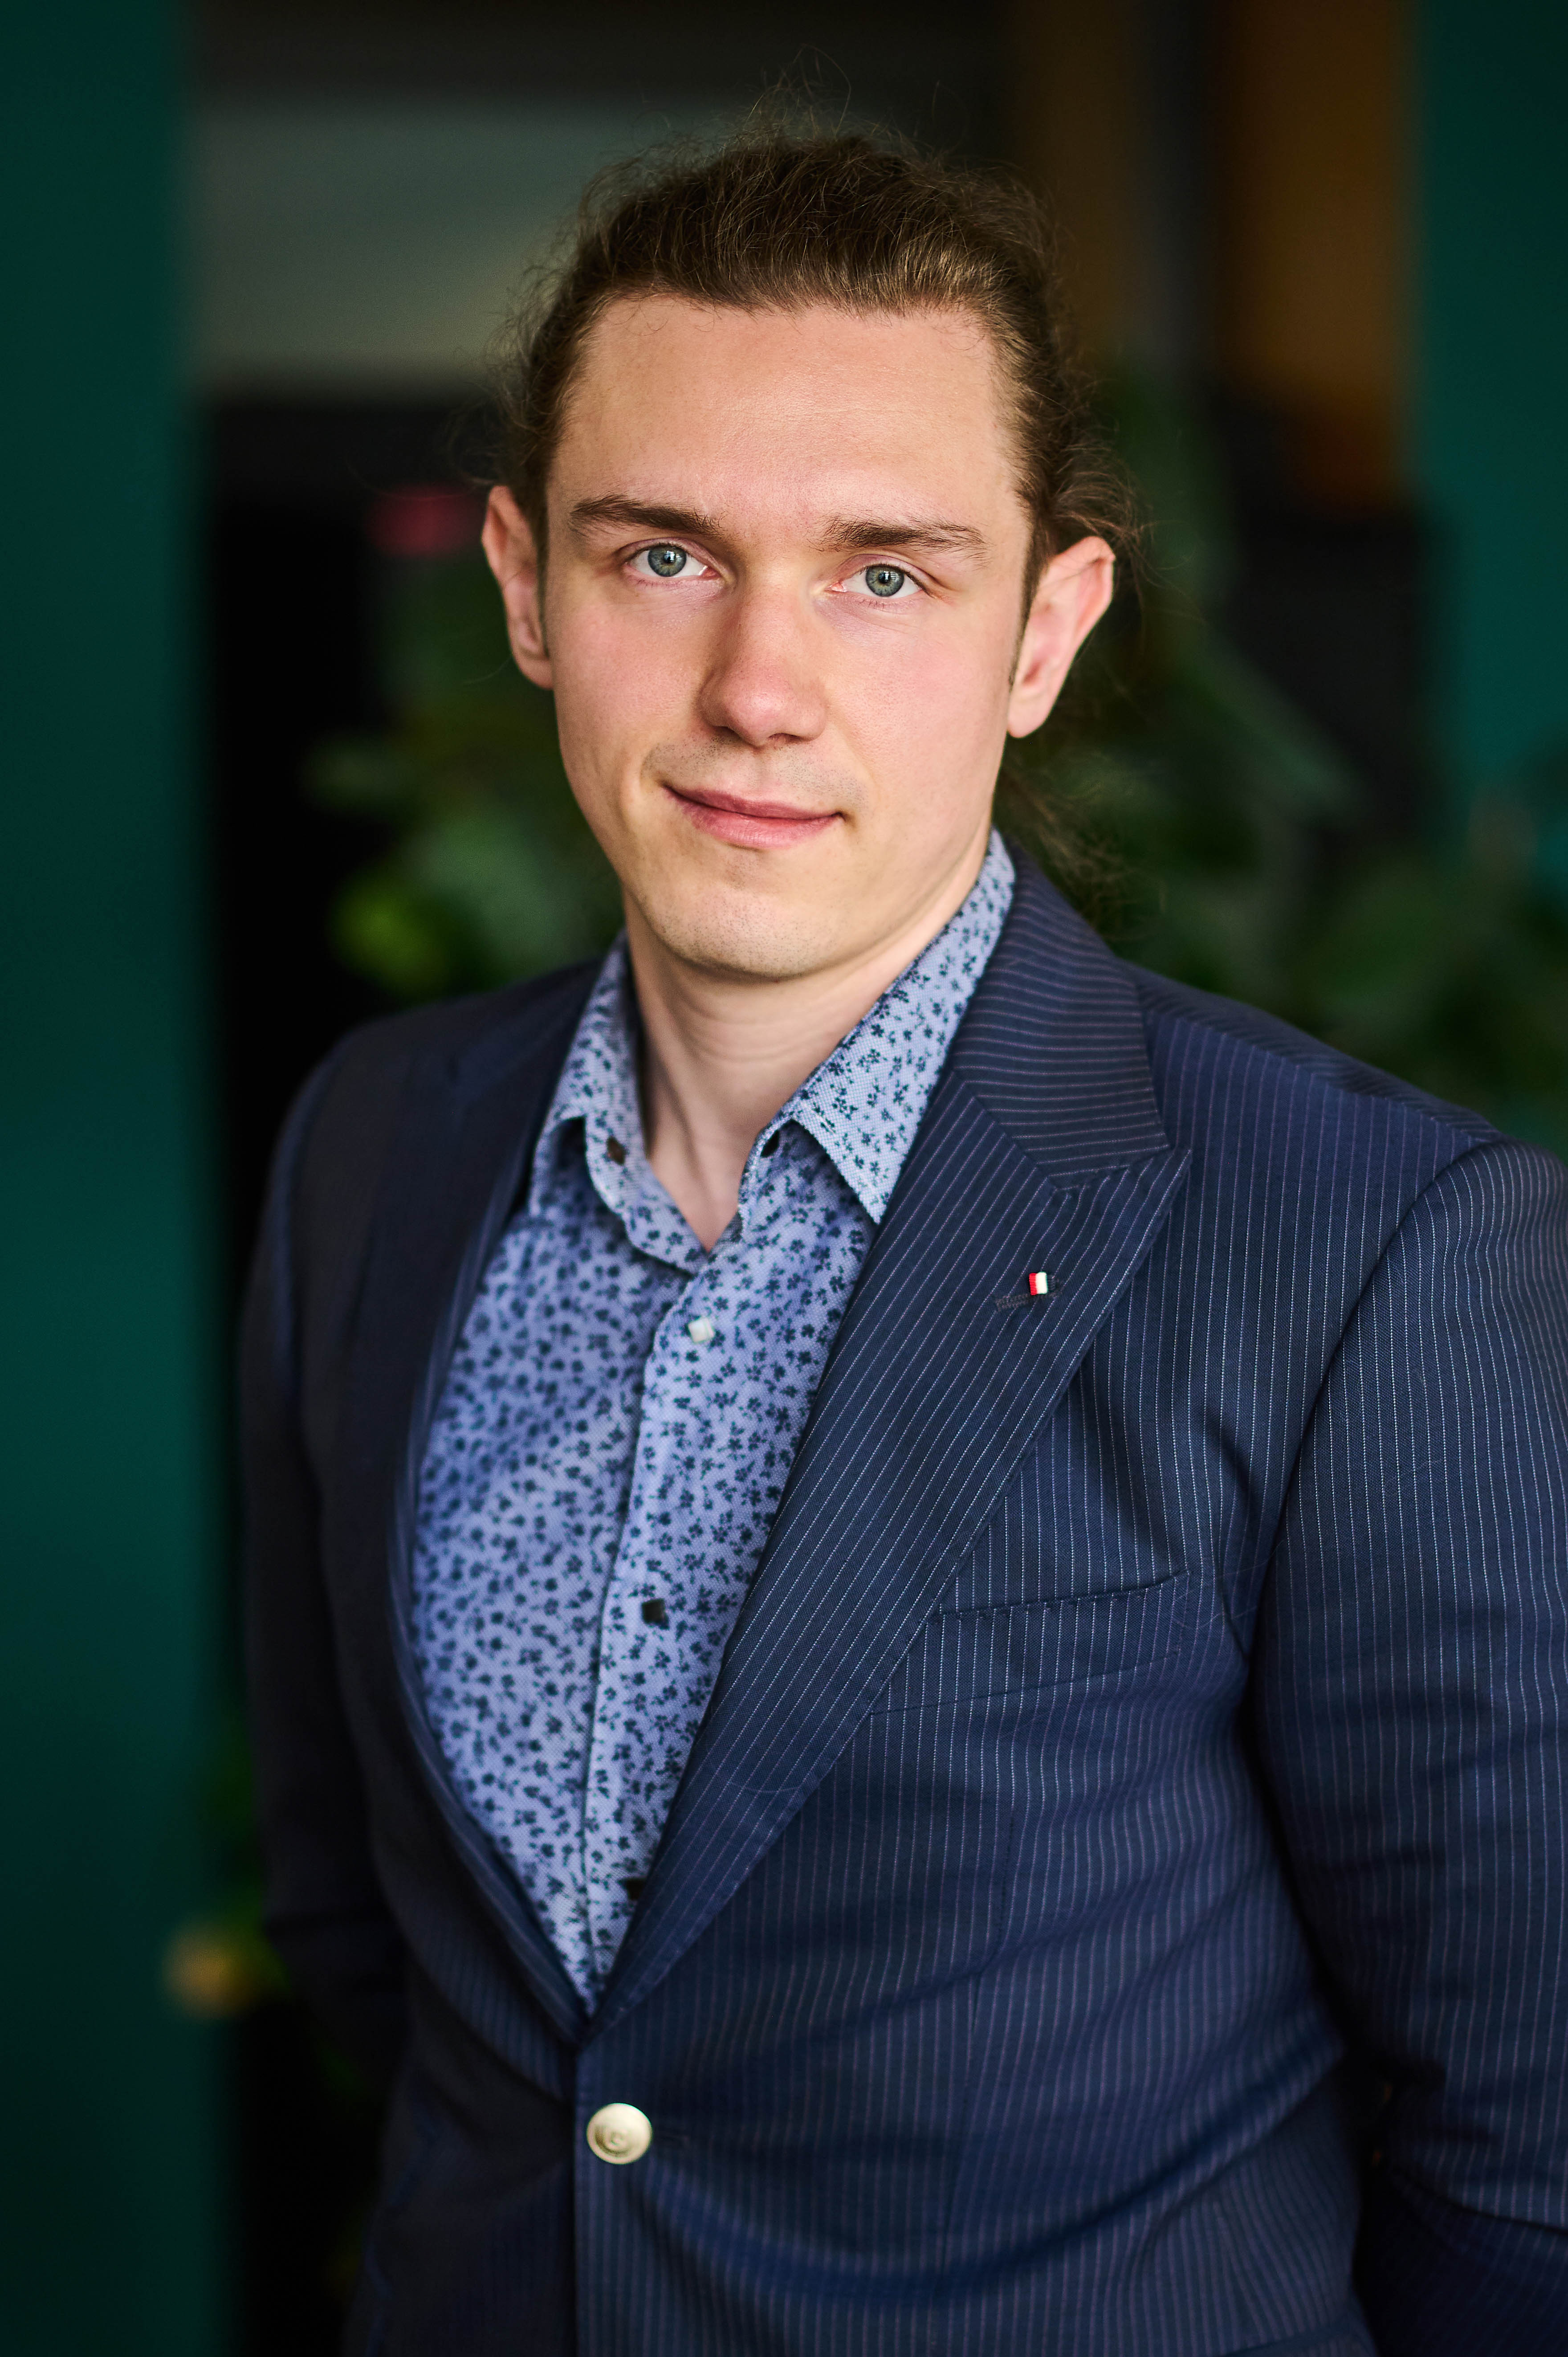
\includegraphics[width=\textwidth]{../manifest/jakub-chojnacki-billennium.jpg} 
    \end{column}
    \begin{column}{0.7\textwidth}
        
\includegraphics[width=0.5\textwidth]{../manifest/logo-ibe.png} 
        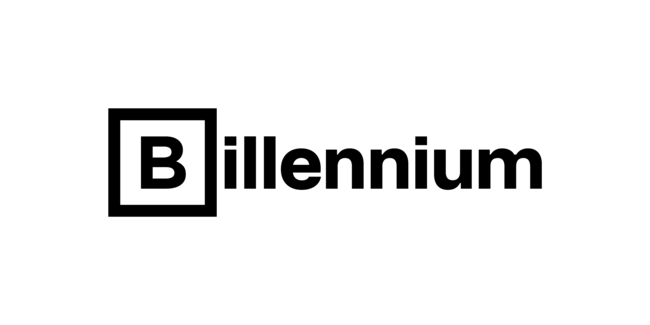
\includegraphics[width=0.5\textwidth]{../manifest/logo-billennium.png}
    \end{column}
\end{columns}
\end{frame}

% -----------------------------
% -------- KONTAKT -------------
% -----------------------------

\begin{frame}
\frametitle{Kontakt}

\begin{columns}
    \begin{column}{0.6\textwidth}
        \begin{itemize}
            \item \textbf{Imię i Nazwisko:} Jakub Chojnacki
            \item \textbf{E-mail:} james@marl.engineering
            \item \textbf{Strona internetowa:} https://www.marl.engineering
        \end{itemize}
    \end{column}

    \begin{column}{0.4\textwidth}
        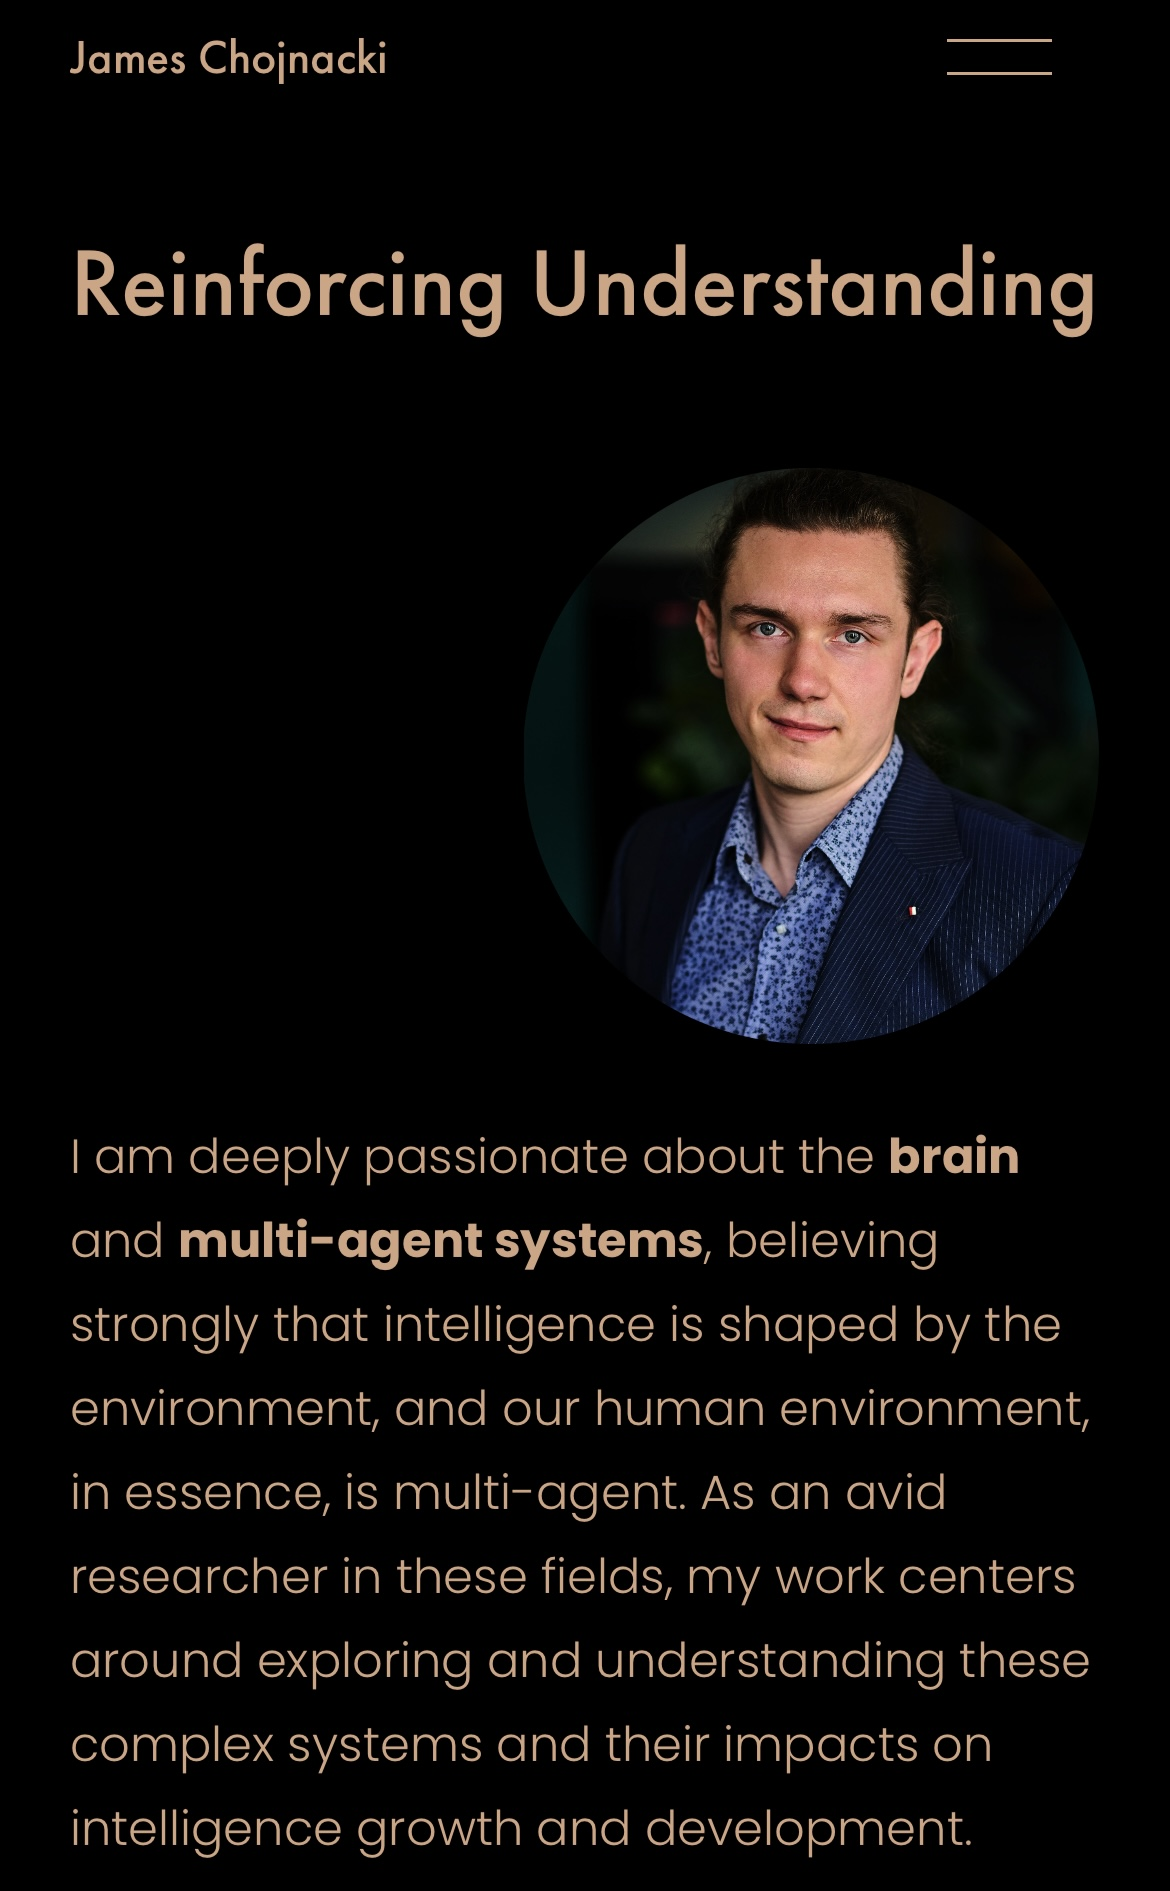
\includegraphics[width=\textwidth]{../manifest/marl-engineering.jpg}
    \end{column}
\end{columns}
\end{frame}

% -----------------------------
% -------- AGENDA -------------
% -----------------------------

\begin{frame}
\frametitle{Agenda}
\begin{enumerate}
    \item Historia i rozwój AI 
    \item Przerwa 
    \item Podstawy maszynowego uczenia i głębokiego uczenia
    \item QA - Sesja pytań i odpowiedzi 
\end{enumerate}
\end{frame}

% -----------------------------
% -------- AGENDA -------------
% -----------------------------

\begin{frame}
\frametitle{Agenda}
\begin{enumerate}
    \item \textbf{\color{black}Historia i rozwój AI}
    \item \color{gray}Przerwa
    \item \color{gray}Podstawy uczenia maszynowego i uczenia głębokiego
    \item \color{gray}QA - Sesja pytań i odpowiedzi
\end{enumerate}
\end{frame}

% -----------------------------
% -------- SLAJD 1 ------------
% -----------------------------

\begin{frame}
\frametitle{Definicja AI}

\begin{columns}
    \begin{column}{0.6\textwidth}
        \begin{itemize}
            \item Sztuczna inteligencja to dziedzina nauki komputerowej.
            \item Uczy maszyny "myśleć" i podejmować decyzje jak ludzie.
            \item Dzięki AI, komputery mogą:
            \begin{itemize}
                \item Rozpoznawać obrazy.
                \item Rozumieć język ludzi.
                \item Grać w gry.
            \end{itemize}
        \end{itemize}
    \end{column}

    \begin{column}{0.4\textwidth}
        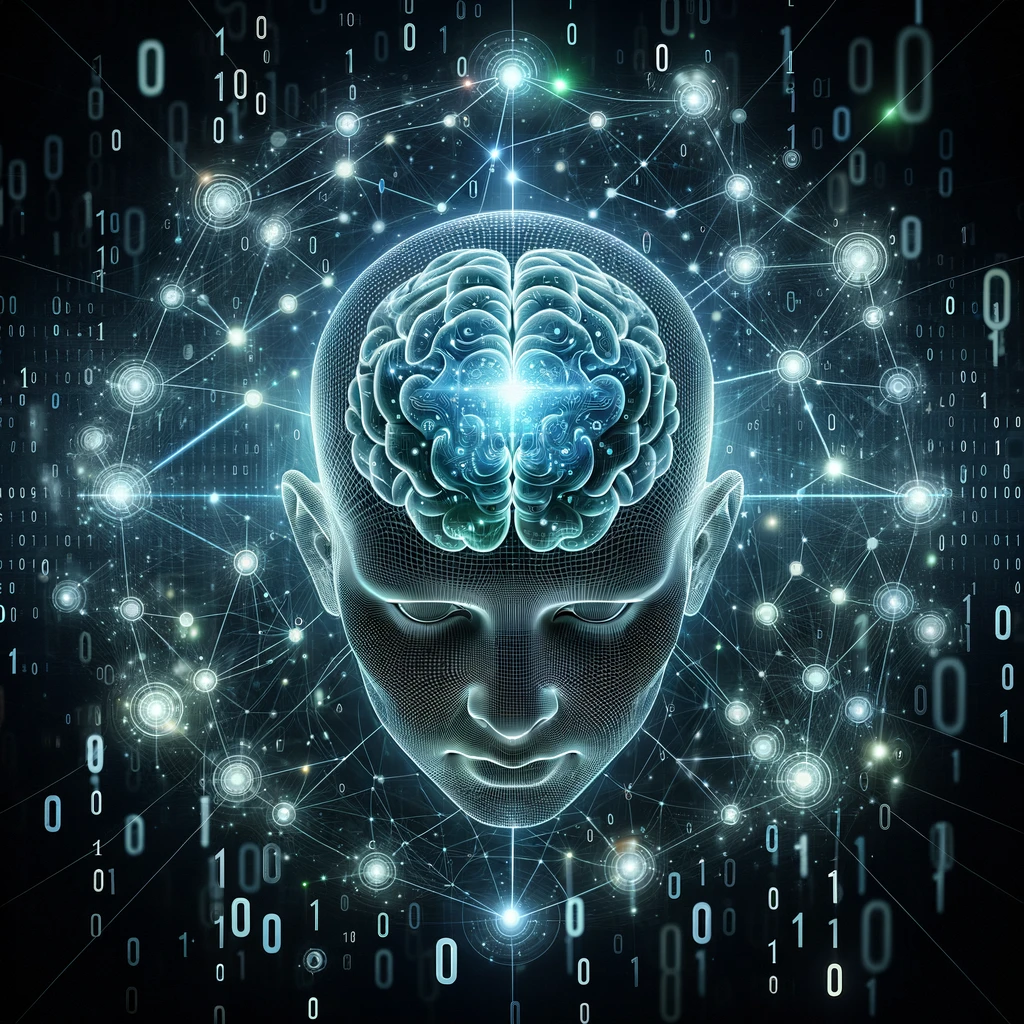
\includegraphics[width=\textwidth]{../manifest/definicja-ai.png}
    \end{column}
\end{columns}
\end{frame}

% -----------------------------
% -------- SLAJD 2 ------------
% -----------------------------

\begin{frame}
\frametitle{Początki myśli o AI}

\begin{columns}
    \begin{column}{0.6\textwidth}
        \begin{itemize}
            \item \textbf{Alan Turing (1940s):}
            \begin{itemize}
                \item "Maszyna Turinga" - podstawy teoretyczne dla komputerów.
                \item Test Turinga - koncepcja oceny inteligencji maszynowej.
            \end{itemize}
            \item \textbf{Claude Shannon (1940s-50s):}
            \begin{itemize}
                \item Twórca teorii informacji.
                \item Badania nad algorytmami genetycznymi i uczeniem maszynowym.
            \end{itemize}
            \item \textbf{John McCarthy (1950s):}
            \begin{itemize}
                \item Wprowadzenie terminu "sztuczna inteligencja".
                \item Twórca języka programowania Lisp, popularnego w badaniach nad AI.
            \end{itemize}
        \end{itemize}
    \end{column}

    \begin{column}{0.4\textwidth}
        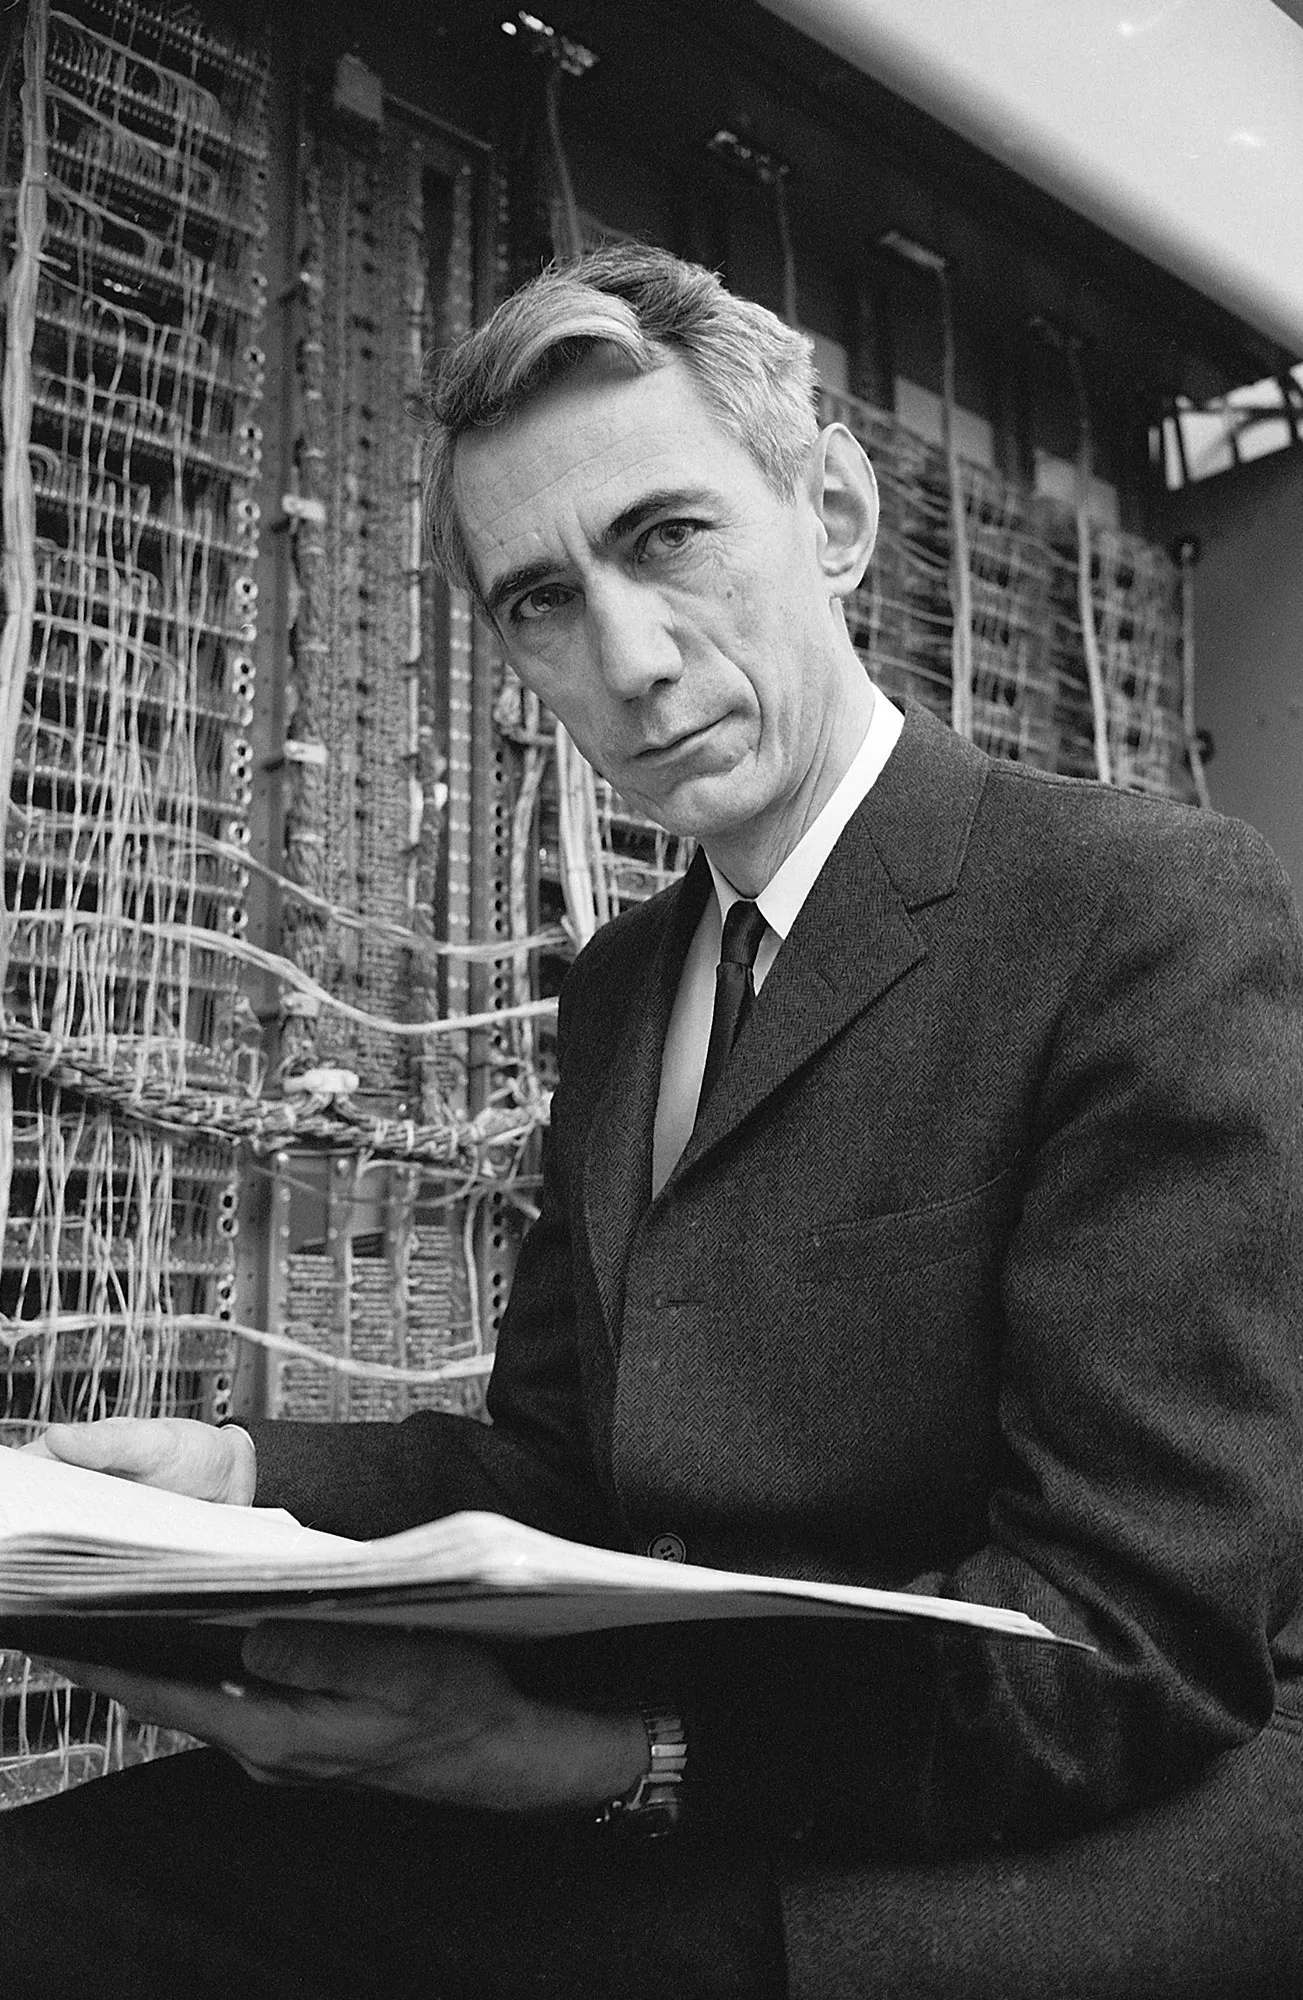
\includegraphics[width=\textwidth]{../manifest/shannon.png}
    \end{column}
\end{columns}
\end{frame}

% -----------------------------
% -------- SLAJD 3 ------------
% -----------------------------

\begin{frame}
\frametitle{Test Turinga}

\begin{columns}
    \begin{column}{0.6\textwidth}
        \begin{itemize}
            \item \textbf{Zaproponowany przez Alana Turinga} w 1950 r. w artykule "Computing Machinery and Intelligence".
            \item \textbf{Pytanie kluczowe:} "Czy maszyny mogą myśleć?"
            \item Test polega na \textbf{konwersacji} między człowiekiem a maszyną ukrytą za ścianą.
            \item Jeśli człowiek \textbf{nie jest w stanie rozróżnić}, czy rozmawia z maszyną czy innym człowiekiem, maszyna "przechodzi" test.
        \end{itemize}
    \end{column}

    \begin{column}{0.4\textwidth}
        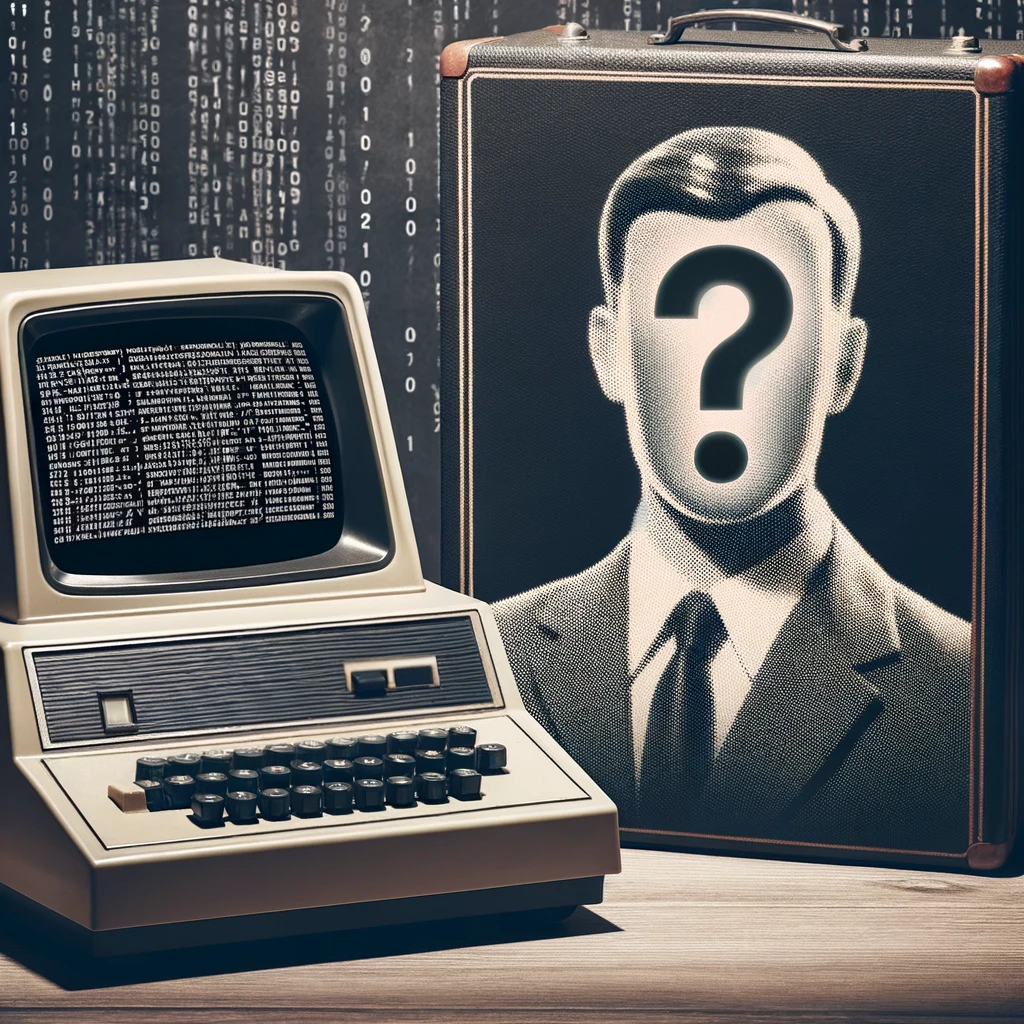
\includegraphics[width=\textwidth]{../manifest/turing-test.png}
    \end{column}
\end{columns}
\end{frame}

% -----------------------------
% -------- SLAJD 4 ------------
% -----------------------------

\begin{frame}
\frametitle{Claude Shannon i Teoria Informacji}

\begin{columns}
    \begin{column}{0.6\textwidth}
        \begin{itemize}
            \item Entropia jest miarą niepewności lub "zaskoczenia" zawartego w danym źródle informacji.
            \item Wysoka entropia oznacza, że informacje są bardziej chaotyczne, nieprzewidywalne lub mają większą zawartość informacji.
            \item Shannon użył entropii do określenia teoretycznych limitów, jak skutecznie można kodować i przesyłać informacje.
        \end{itemize}
    \end{column}

    \begin{column}{0.4\textwidth}
        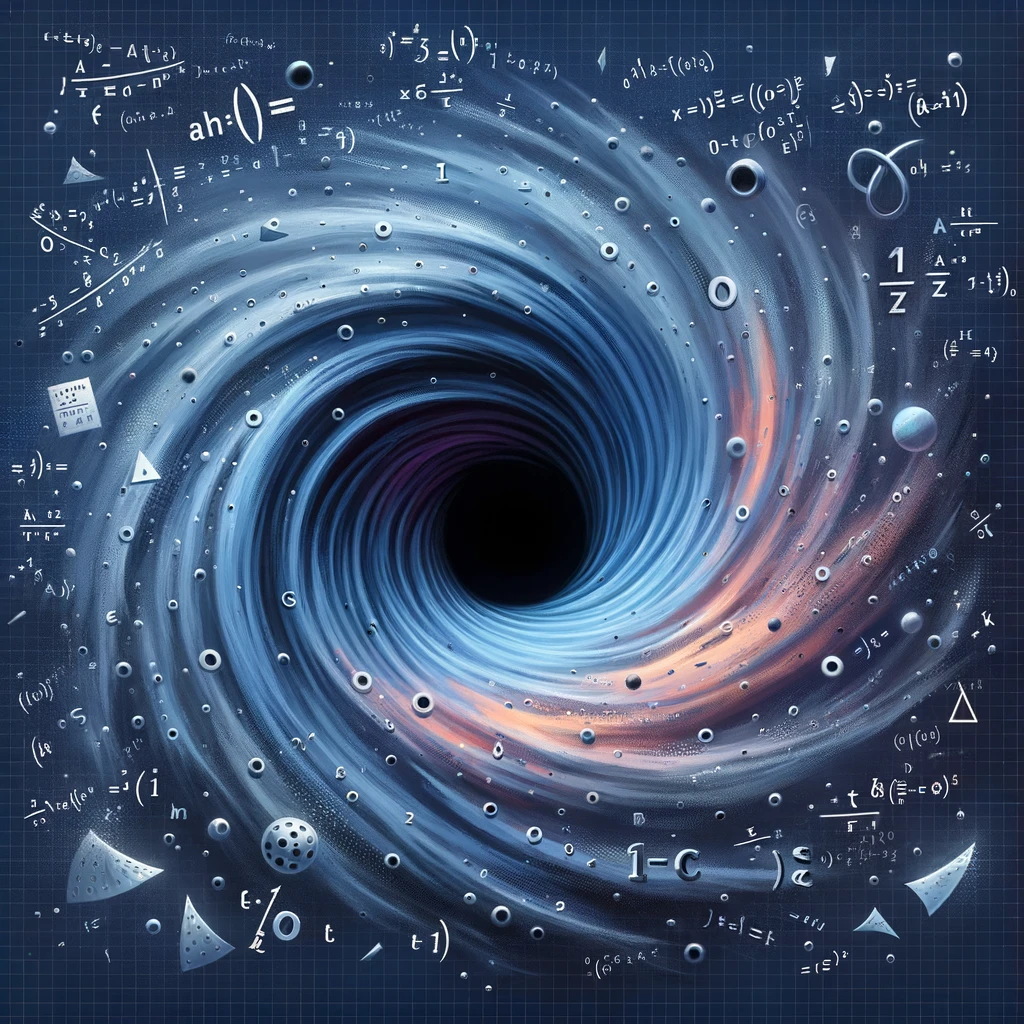
\includegraphics[width=\textwidth]{../manifest/entropy.png} % Zastąp odpowiednim obrazem Claude'a Shannon'a
    \end{column}
\end{columns}
\end{frame}

% -----------------------------
% -------- SLAJD 5 ------------
% -----------------------------

\begin{frame}
\frametitle{John McCarthy i LISP}

\begin{columns}
    \begin{column}{0.6\textwidth}
        \begin{itemize}
            \item McCarthy wymyślił słowo "sztuczna inteligencja" w 1955 roku.
            \item W 1958 roku stworzył język programowania LISP, który stał się popularny w tworzeniu oprogramowania AI.
            \item LISP pozwalał programistom łatwo manipulować symbolami i listami, co było nowością.
            \item McCarthy użył LISP-a do budowania programów, które mogły rozwiązywać problemy matematyczne i logiczne.
        \end{itemize}
    \end{column}

    \begin{column}{0.4\textwidth}
        
\includegraphics[width=\textwidth]{../manifest/lisp.png} 
    \end{column}
\end{columns}
\end{frame}

% -----------------------------
% -------- SLAJD 6 ------------
% -----------------------------

\begin{frame}
\frametitle{Era Symboliki w AI}

\begin{columns}
    \begin{column}{0.6\textwidth}
        \begin{itemize}
            \item To były początki AI, głównie lata 50., 60. i 70. XX wieku.
            \item Ludzie próbowali nauczyć komputery „myślenia” poprzez używanie symboli i reguł, jak w grze szachowej.
            \item Zbudowali „inteligentne” programy, które mogły rozwiązywać łamigłówki i zagadki, używając zasad i instrukcji.
            \item Celem było, aby komputer używał tych reguł, aby sam znaleźć odpowiedzi na pytania i rozwiązać problemy.
        \end{itemize}
    \end{column}

    \begin{column}{0.4\textwidth}
        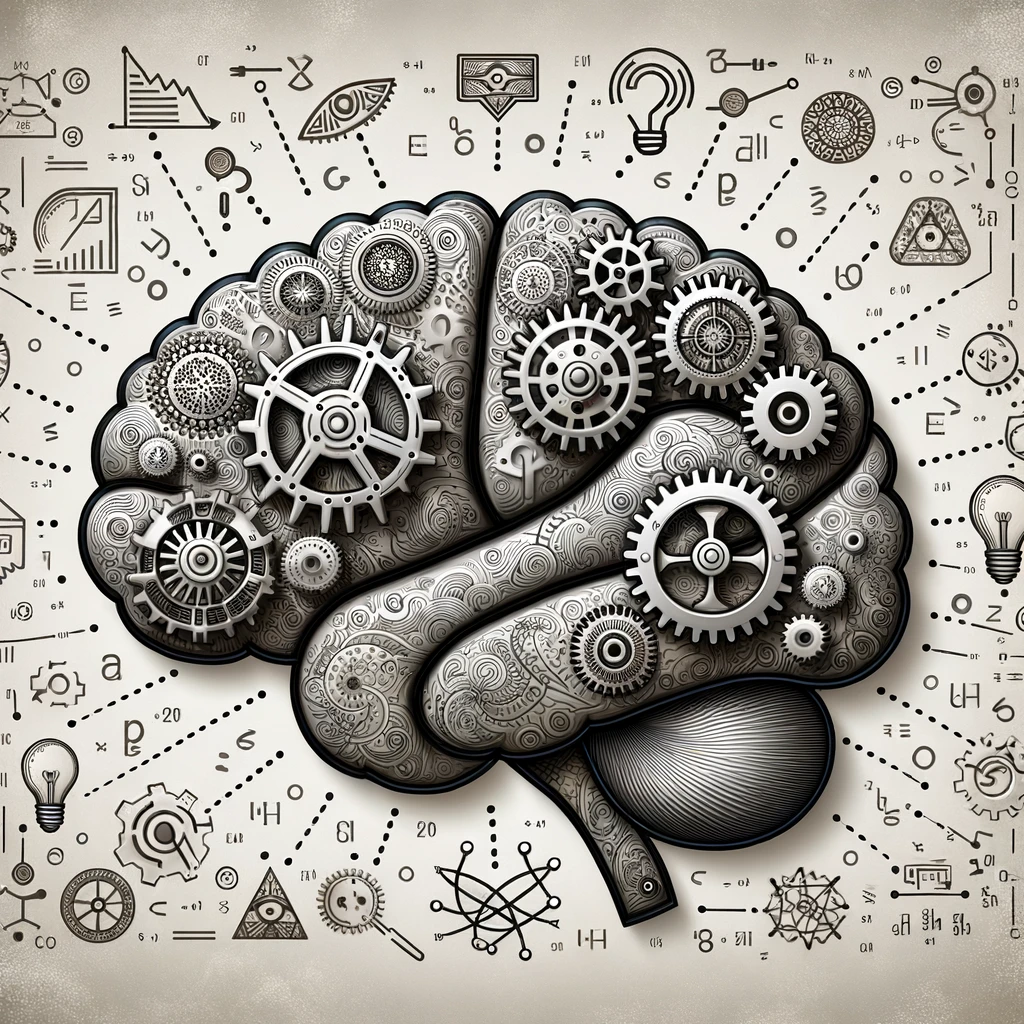
\includegraphics[width=\textwidth]{../manifest/gofai.png} % Wstaw odpowiedni obrazek
    \end{column}
\end{columns}
\end{frame}

% -----------------------------
% -------- SLAJD 7 ------------
% -----------------------------

\begin{frame}
\frametitle{Wzloty i Upadki AI}

\begin{columns}
    \begin{column}{0.6\textwidth}
        \begin{itemize}
            \item \textbf{Wzloty:}
            \begin{itemize}
                \item Lata 50. i 60.: Dużo optymizmu, pierwsze programy grające w szachy, rozpoznające obrazy.
                \item Lata 80.: Boom na ekspertowe systemy komputerowe, które pomagały lekarzom i inżynierom w rozwiązywaniu problemów.
            \end{itemize}
            \item \textbf{Upadki („Zimy AI”):}
            \begin{itemize}
                \item Lata 70.: Brak postępów, problemy techniczne, cięcia finansowania.
                \item Lata 90.: Konkurencja z innymi technologiami, mniej funduszy na badania.
            \end{itemize}
        \end{itemize}
    \end{column}

    \begin{column}{0.4\textwidth}
        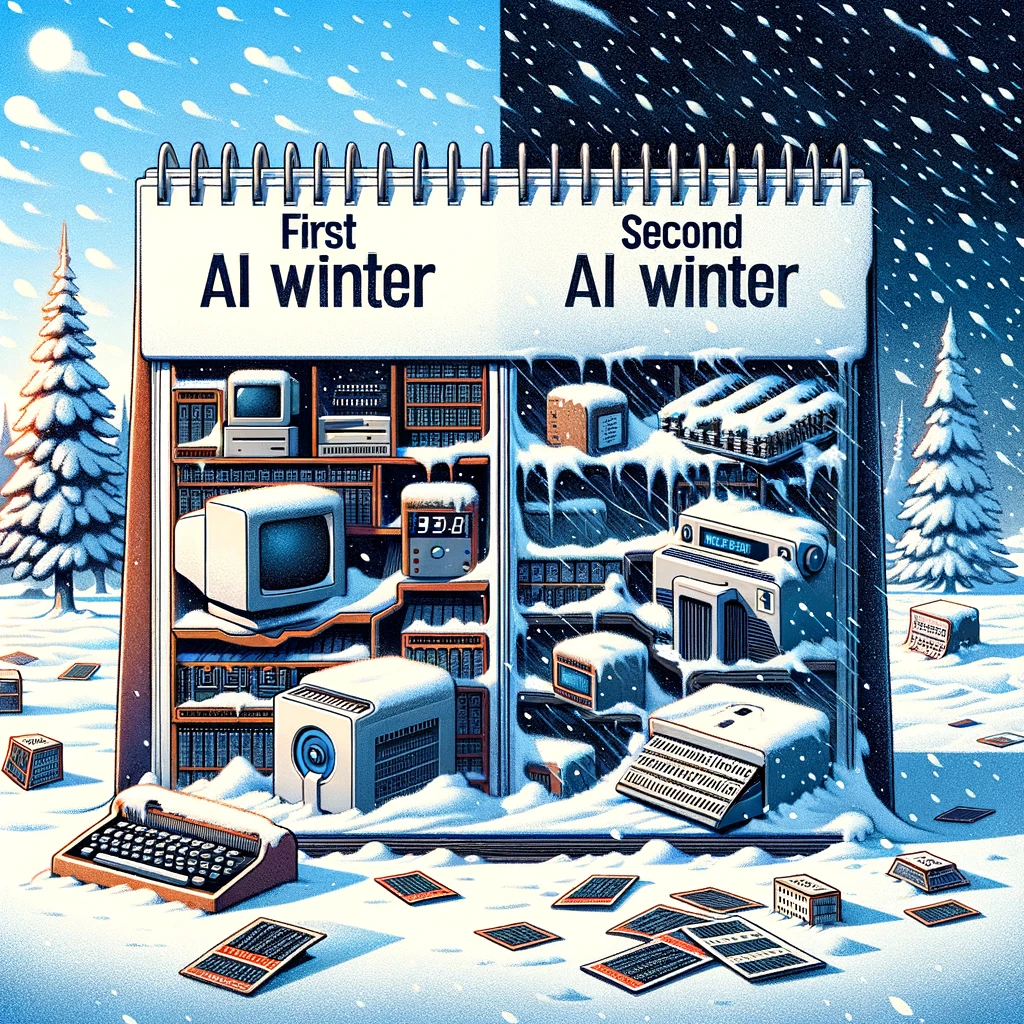
\includegraphics[width=\textwidth]{../manifest/ai-winter.png}
    \end{column}
\end{columns}
\end{frame}

% -----------------------------
% -------- SLAJD 8 ------------
% -----------------------------

\begin{frame}
\frametitle{Zimy AI}
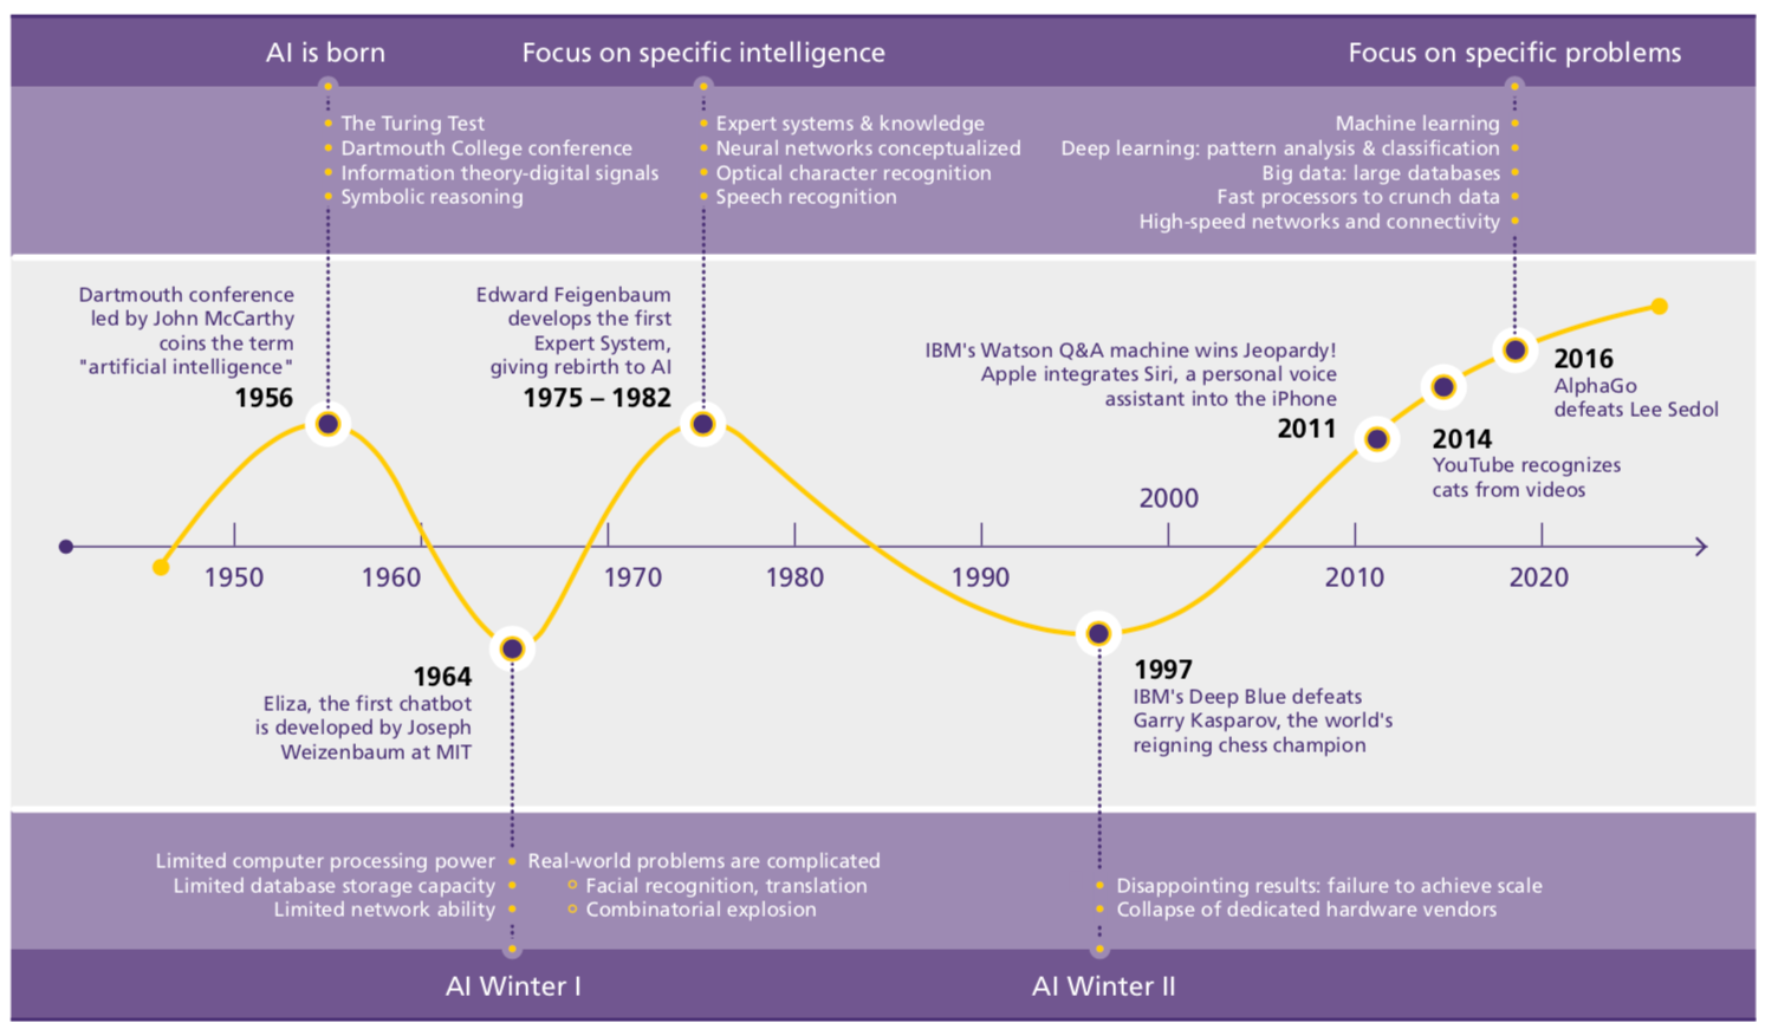
\includegraphics[width=\textwidth,height=\textheight,keepaspectratio]{../manifest/ai-winter-plot.png}
\end{frame}

% -----------------------------
% -------- SLAJD 9 ------------
% -----------------------------

\begin{frame}
\frametitle{Eksplozja AI}
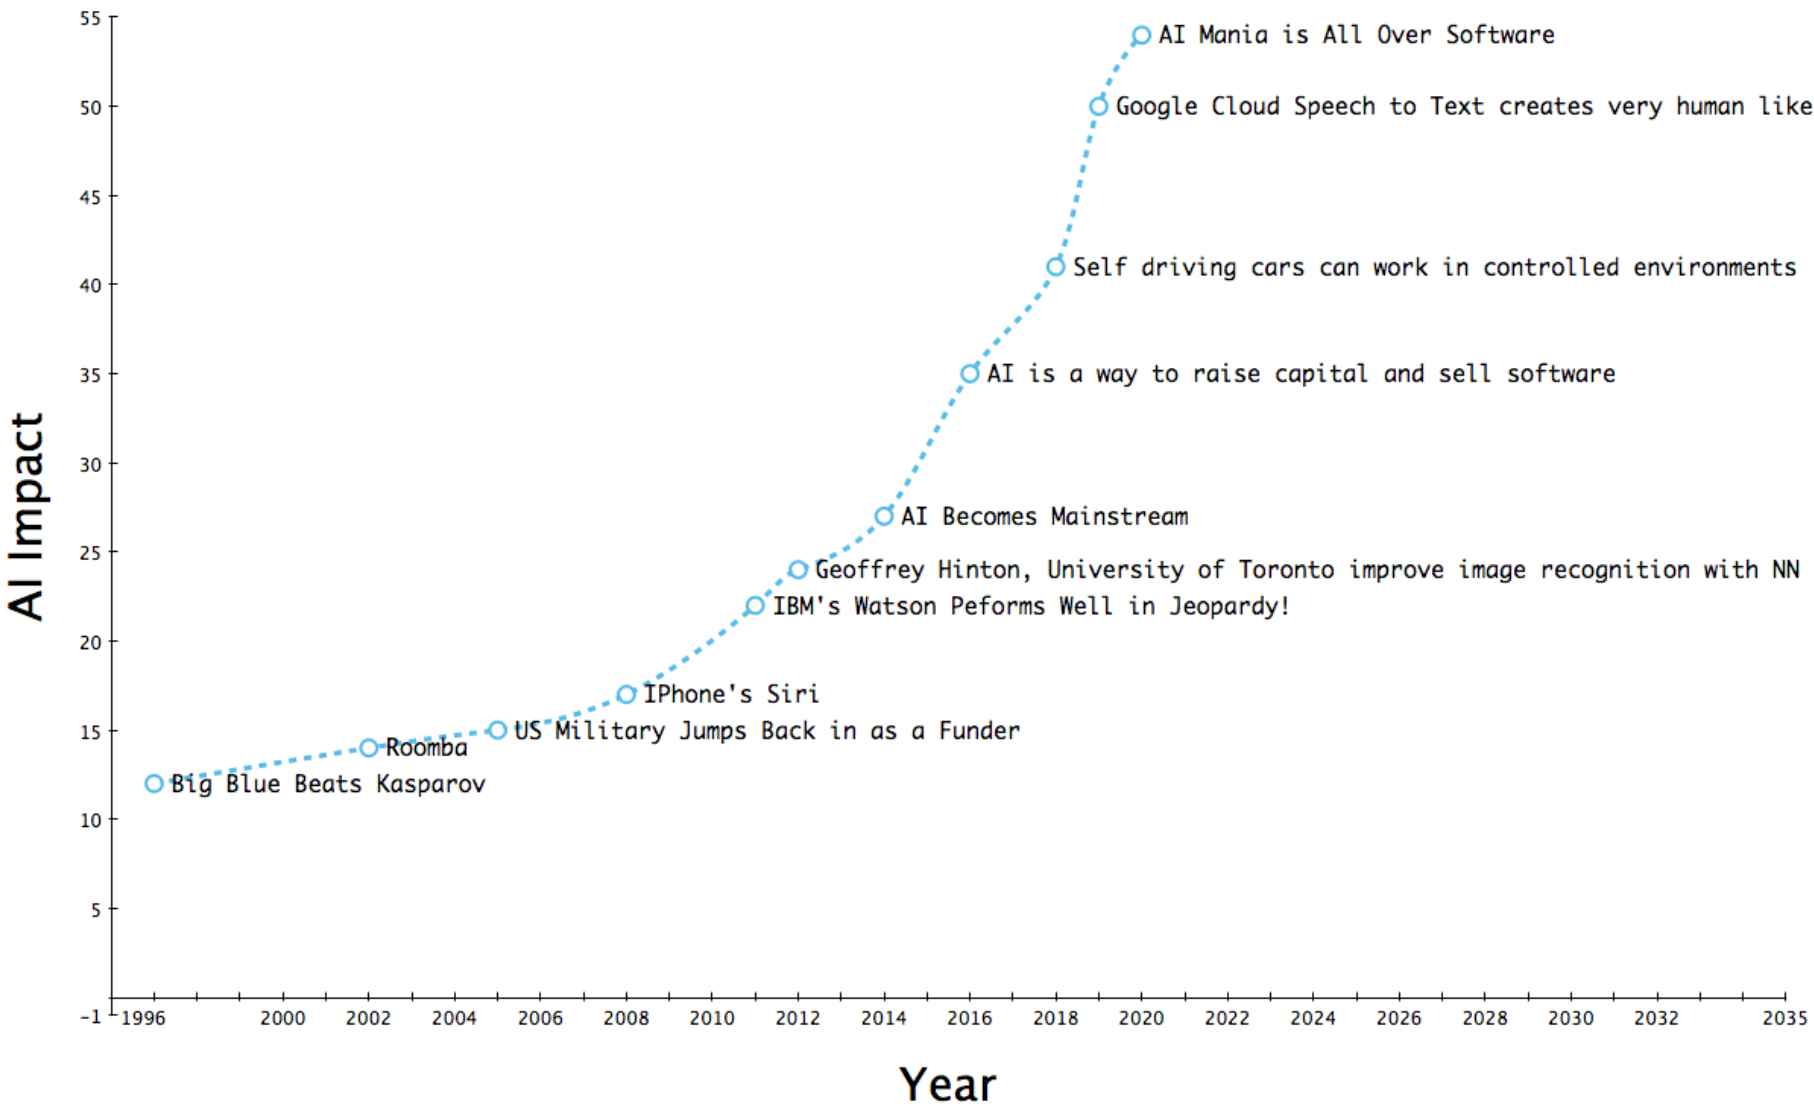
\includegraphics[width=\textwidth,height=\textheight,keepaspectratio]{../manifest/new-hope.png}
\end{frame}

% -----------------------------
% -------- SLAJD 10 ------------
% -----------------------------

\begin{frame}
\frametitle{Co przyczyniło się do eksplozji AI po latach 90?}

\begin{itemize}
    \item Rozwój i ekspansja internetu
    \item Wzrost dostępnych danych cyfrowych
    \item Rozwój nowych algorytmów uczenia maszynowego
    \item Ulepszenia technologiczne i mocniejsze komputery
\end{itemize}

\end{frame}

% -----------------------------
% -------- SLAJD 11 ------------
% -----------------------------

\begin{frame}
\frametitle{Co przyczyniło się do eksplozji AI po latach 90?}

\begin{itemize}
    \item[\textcolor{green}{\checkmark}] Rozwój i ekspansja internetu
    \item[\textcolor{green}{\checkmark}] Wzrost dostępnych danych cyfrowych
    \item[\textcolor{green}{\checkmark}] Rozwój nowych algorytmów uczenia maszynowego
    \item[\textcolor{green}{\checkmark}] Ulepszenia technologiczne i mocniejsze komputery
\end{itemize}

\end{frame}

% -----------------------------
% -------- SLAJD 12 ------------
% -----------------------------

\begin{frame}
\frametitle{Wzrost danych cyfrowych w zetabajtach (\(10^{21}\))}
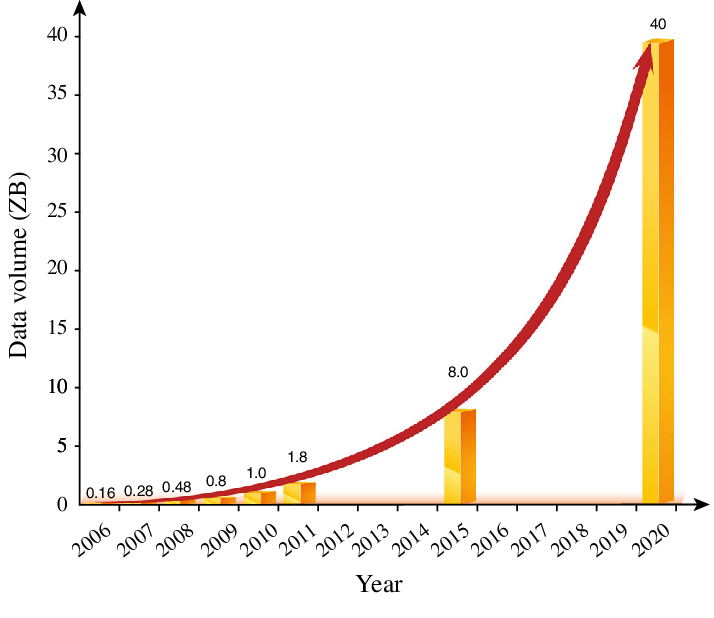
\includegraphics[width=\textwidth,height=0.8\textheight,keepaspectratio]{../manifest/data-growth.png}
\end{frame}

% -----------------------------
% -------- SLAJD 13 ------------
% -----------------------------

\begin{frame}
\frametitle{Eksplozja danych wideo w internecie}

\begin{columns}
    \begin{column}{0.6\textwidth}
        \begin{itemize}
            \item Co minutę na internet trafia \textbf{500 godzin materiału wideo}.
            \item Około \textbf{11 miliardów TikToków} jest przesyłanych co rok na platformę.
        \end{itemize}
    \end{column}

    \begin{column}{0.4\textwidth}
        
\includegraphics[width=\textwidth]{../manifest/tt.png} % Wstaw ścieżkę do zdjęcia
    \end{column}
\end{columns}
\end{frame}

% -----------------------------
% -------- SLAJD 14 ------------
% -----------------------------

\begin{frame}
\frametitle{Ogrom danych na platformie TikTok}

\begin{columns}
    \begin{column}{0.6\textwidth}
        \begin{itemize}
            \item Każdego dnia dodawanych jest \textcolor{red}{33 miliony} nowych TikToków,
            \item Jeśli każdy TikTok trwa średnio 1 minute
            \item \textbf{To jednemu człowiekowi zajęłoby ponad \textcolor{red}{400 lat nieprzerwanego oglądania}, aby zobaczyć wszystkie TikToki dodane TYLKO dzisiaj na platforme.}
        \end{itemize}
    \end{column}
    
    \begin{column}{0.4\textwidth}
        
\includegraphics[width=\textwidth]{../manifest/human-tiktok.png} 
    \end{column}
\end{columns}
\end{frame}

% -----------------------------
% -------- SLAJD 15 ------------
% -----------------------------

\begin{frame}
\frametitle{Rozwój algorytmów uczenia maszynowego w latach 90.}

\begin{columns}
    \begin{column}{0.6\textwidth}
        \begin{itemize}
            \item Algorytmy takie jak Support Vector Machines (SVM) i Random Forests zyskały popularność dzięki swojej elastyczności i mocnemu matematycznemu podłożu.
            \item Mimo że sieci neuronowe były już znane, ich zastosowanie wymagało zbyt dużego nakładu mocy obliczeniowej.
        \end{itemize}
    \end{column}

    \begin{column}{0.4\textwidth}
        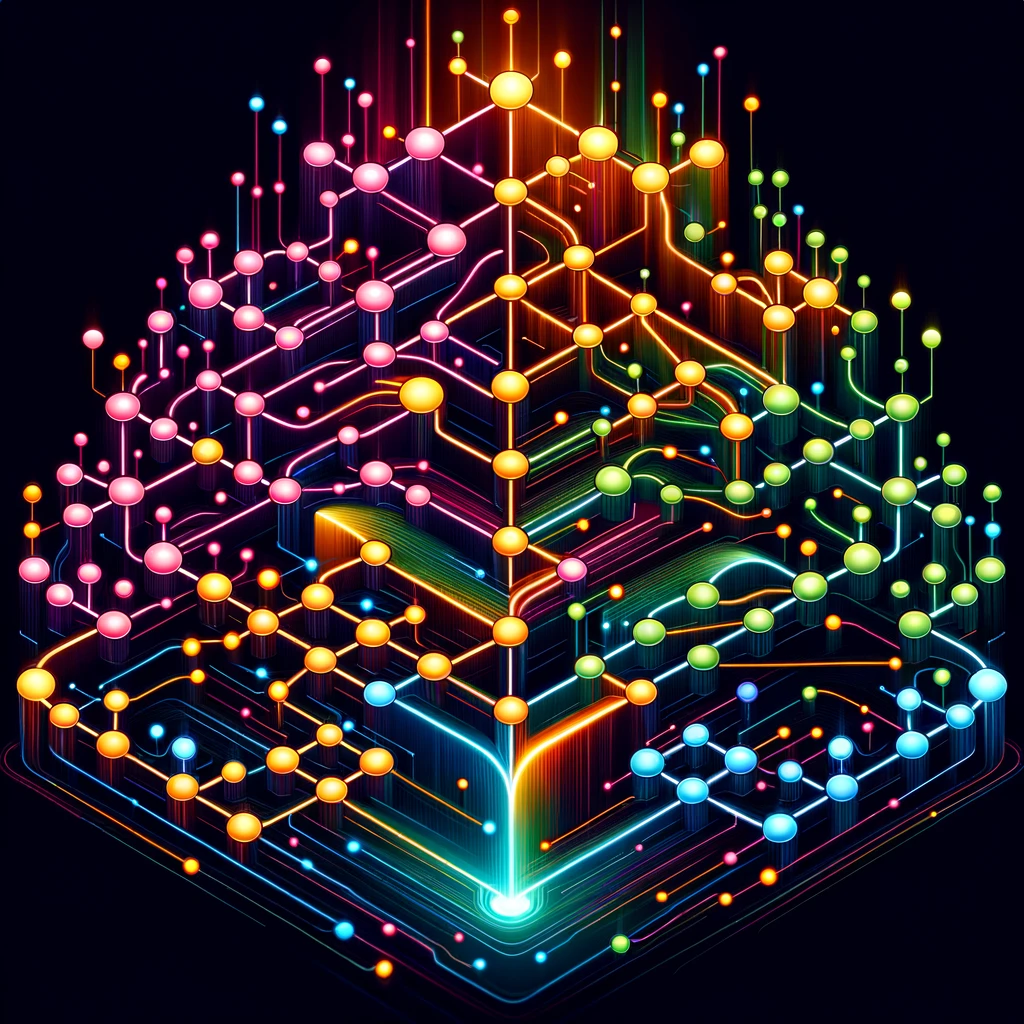
\includegraphics[width=\textwidth]{../manifest/random-forest.png}
    \end{column}
\end{columns}
\end{frame}

% -----------------------------
% -------- SLAJD 16 ------------
% -----------------------------

\begin{frame}
\frametitle{Ulepszenia technologiczne i mocniejsze komputery}

\begin{columns}
    \begin{column}{0.6\textwidth}
        \begin{itemize}
            \item \textbf{Karty graficzne (GPU):} Ulepszony hardware graficzny, który okazał się być wyjątkowo efektywny w przyspieszaniu obliczeń wymaganych w algorytmach głębokiego uczenia.
            \item \textbf{Era Deep Learning:} Rozwój GPU w latach 2000. umożliwił powstanie i szybki rozwój głębokiego uczenia, revolutionizując dziedziny takie jak rozpoznawanie obrazów i przetwarzanie języka naturalnego.
        \end{itemize}
    \end{column}

    \begin{column}{0.4\textwidth}
        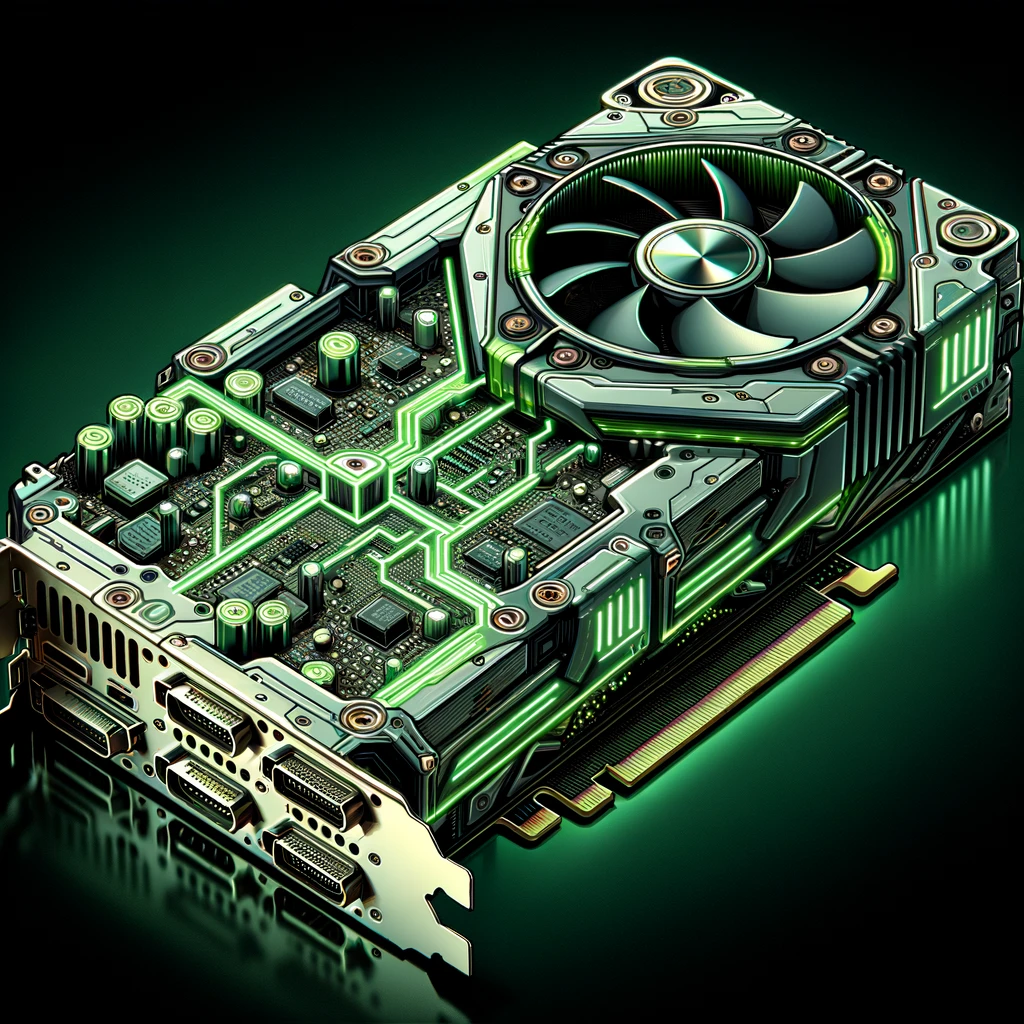
\includegraphics[width=\textwidth]{../manifest/nvidia-gpu.png} % Wstaw ścieżkę do zdjęcia ilustrującego karty graficzne (GPU)
    \end{column}
\end{columns}
\end{frame}

% -----------------------------
% -------- SLAJD 17 ------------
% -----------------------------

\begin{frame}
\frametitle{Karty graficzne (GPU) a głębokie uczenie}

\begin{columns}
    \begin{column}{0.6\textwidth}
        \begin{itemize}
            \item \textbf{CPU:}
                \begin{itemize}
                    \item Zoptymalizowany do zarządzania systemem i koordynowania pracy różnych części komputera.
                    \item Specjalizuje sie w zadanich wymagających trudnych obliczeń.
                \end{itemize}
            \item \textbf{GPU:}
                \begin{itemize}
                    \item Specjalizuje się w wykonywaniu wielu obliczeń matematycznych jednocześnie.
                    \item Idealny do zadań związanych z głębokim uczeniem, które wymagają dużej ilości prostych operacji matematycznych.
                \end{itemize}
        \end{itemize}
    \end{column}

    \begin{column}{0.4\textwidth}
        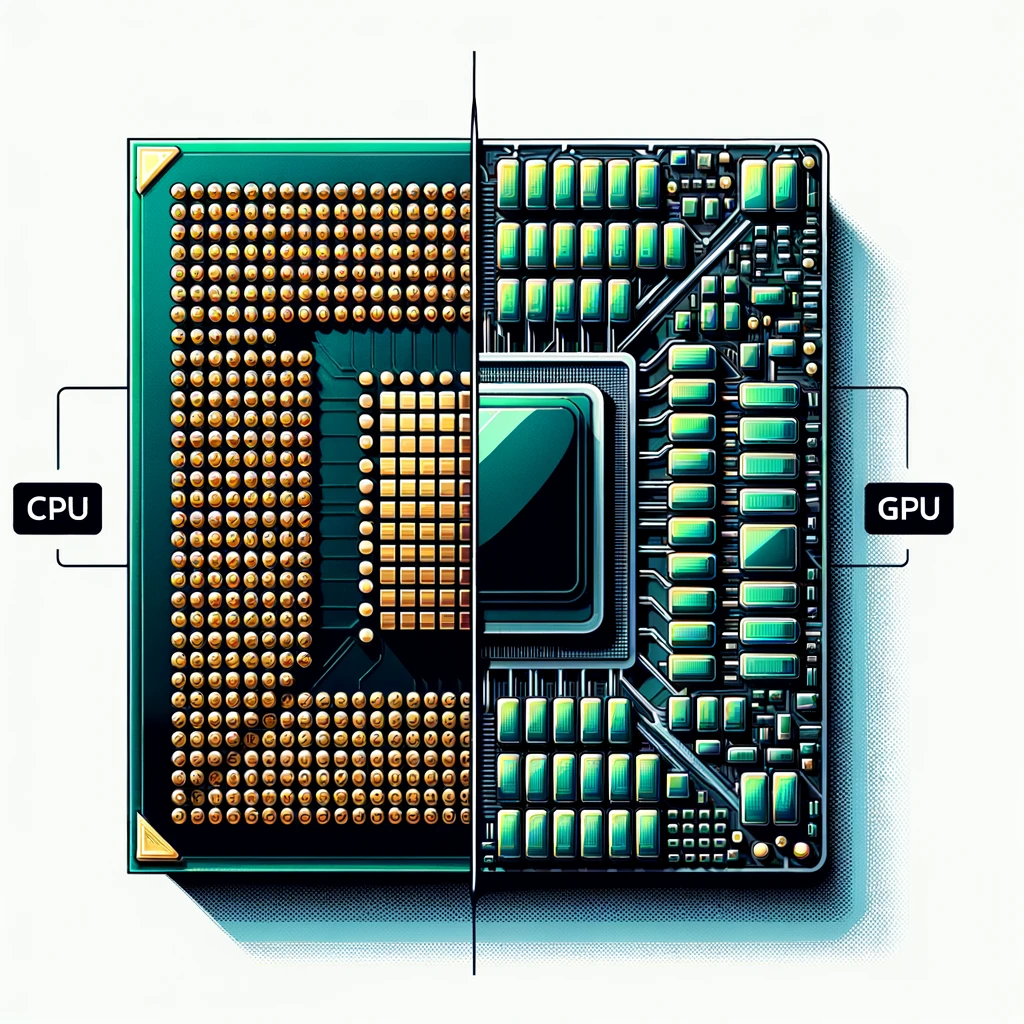
\includegraphics[width=\textwidth]{../manifest/cpu-gpu.png}
    \end{column}
\end{columns}
\end{frame}

% -----------------------------
% -------- SLAJD 18 ------------
% -----------------------------

\begin{frame}
\frametitle{GPU: Klucz do przejścia od Machine Learning do Deep Learning}

\begin{itemize}
    \item \textbf{Proste operacje:} Głębokie uczenie, zwłaszcza sieci neuronowe, polega głównie na prostych operacjach matematycznych takich jak dodawanie i mnożenie.
    \item \textbf{Więcej rdzeni w GPU:} Karty graficzne mają znacznie więcej rdzeni niż procesory CPU. Na przykład, nowoczesne GPU mogą mieć nawet 5000 rdzeni, podczas gdy typowe CPU może mieć do 32 rdzeni.
    \item \textbf{Wpływ na Deep Learning:} Wykorzystanie GPU umożliwiło naukowcom trenowanie głębokich i złożonych modeli, co było trudne do osiągnięcia przy użyciu tylko CPU.
\end{itemize}

\end{frame}

% -----------------------------
% -------- SLAJD 19 -----------
% -----------------------------

\begin{frame}
\frametitle{Perceptron}
    \begin{figure}
        \centering
        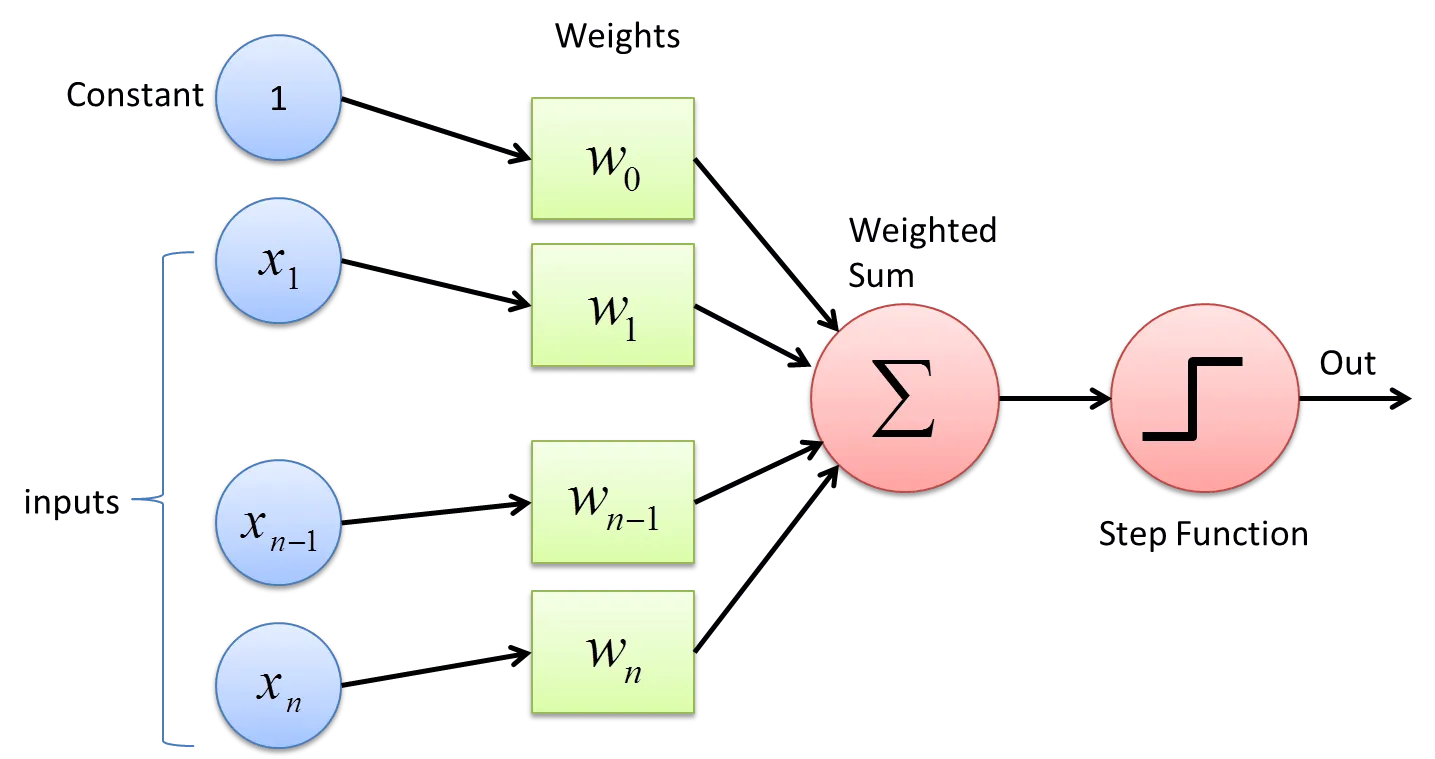
\includegraphics[width=\textwidth,height=\textheight,keepaspectratio]{../manifest/perceptron.png}
    \end{figure}
\end{frame}

% -----------------------------
% -------- SLAJD 20 ----------
% -----------------------------

\begin{frame}
\frametitle{Sieć Neuronowa (wiele perceptronów)}
    \begin{figure}
        \centering
        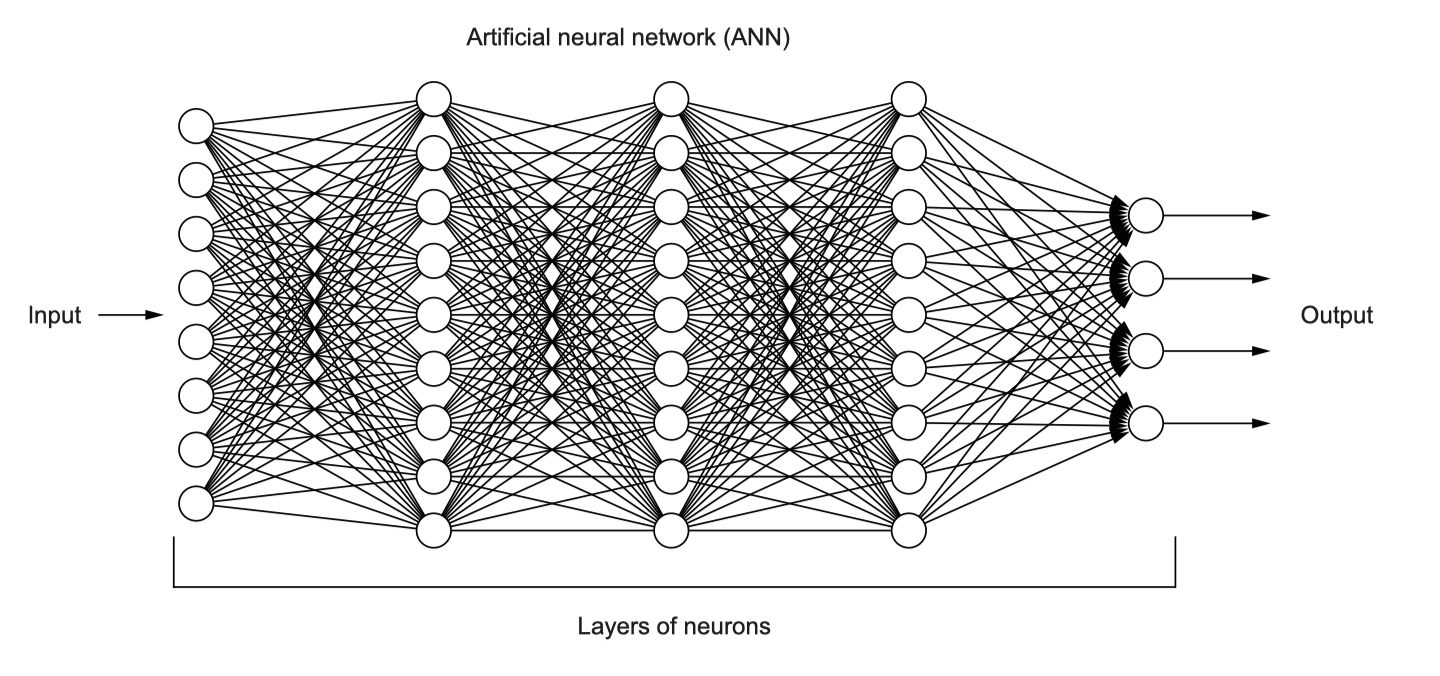
\includegraphics[width=\textwidth,height=\textheight,keepaspectratio]{../manifest/mlp.png}
    \end{figure}
\end{frame}

% -----------------------------
% -------- SLAJD 21 ----------
% -----------------------------

\begin{frame}
\frametitle{Jak działają sieci neuronowe?}

\begin{columns}
    \begin{column}{0.5\textwidth}
        \begin{itemize}
            \item Sieci neuronowe używają "neuronów" połączonych "wagami", które działają jak przełączniki.
            \item Wagi "sterują" tym, jak silny jest wpływ jednego neuronu na drugi.
            \item Sieć "uczy się" poprzez dostosowywanie tych wag, tak aby lepiej przewidywać odpowiedzi na podstawie danych wejściowych.
        \end{itemize}
    \end{column}

    \begin{column}{0.5\textwidth}
        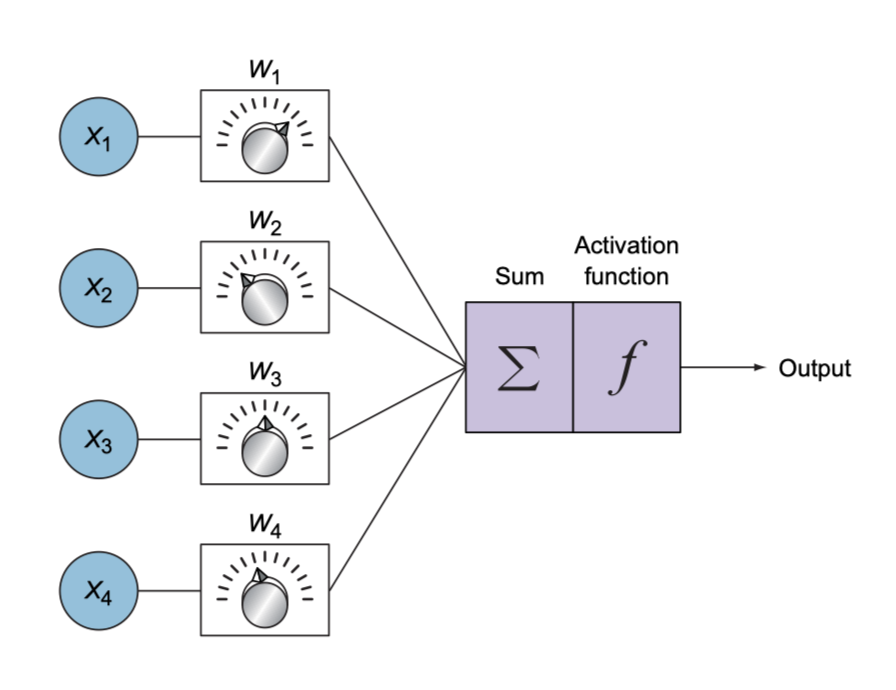
\includegraphics[width=\textwidth]{../manifest/nn-switch.png} % Wstaw ścieżkę do twojego obrazu
    \end{column}
\end{columns}

\end{frame}

% -----------------------------
% -------- SLAJD 22 ----------
% -----------------------------

\begin{frame}
\frametitle{Sieć Neuronowa (wiele perceptronów)}
    \begin{figure}
        \centering
        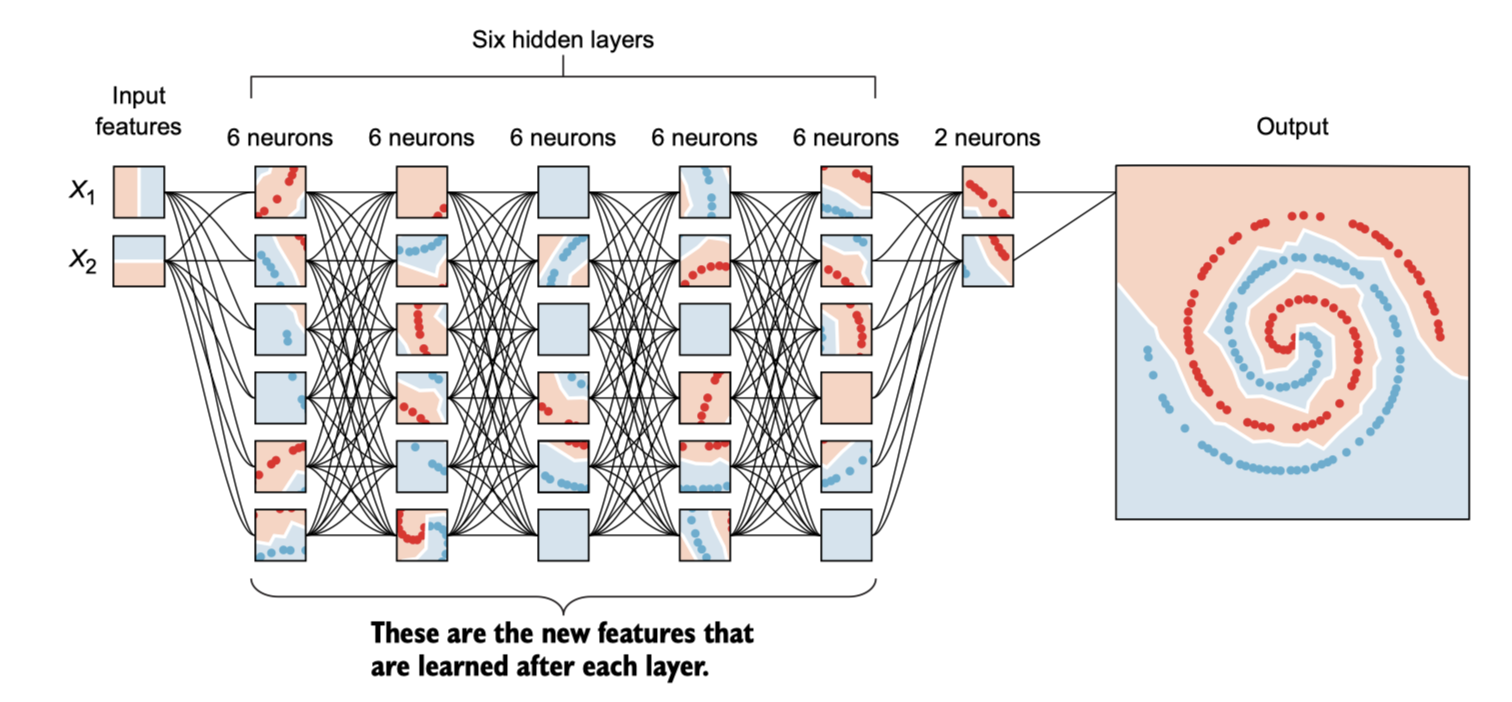
\includegraphics[width=\textwidth,height=\textheight,keepaspectratio]{../manifest/mlp-features.png}
    \end{figure}
\end{frame}

% -----------------------------
% -------- SLAJD 23 ----------
% -----------------------------

\begin{frame}
\frametitle{Cechy (features)}
    \begin{figure}
        \centering
        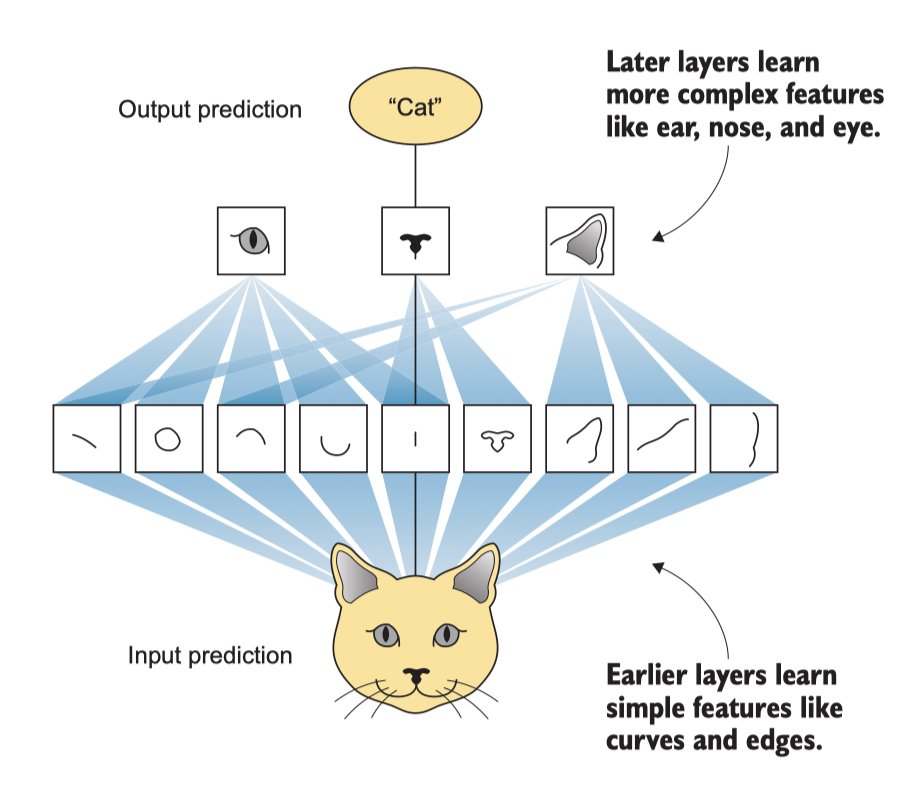
\includegraphics[width=\textwidth,height=0.7\textheight,keepaspectratio]{../manifest/cat.png}
    \end{figure}
\end{frame}

% -----------------------------
% -------- AGENDA -------------
% -----------------------------

\begin{frame}
\frametitle{Agenda}
\begin{enumerate}
    \item \color{gray}Historia i rozwój AI
    \item \textbf{\color{black}Przerwa}
    \item \color{gray}Podstawy uczenia maszynowego i uczenia głębokiego
    \item \color{gray}QA - Sesja pytań i odpowiedzi
\end{enumerate}
\end{frame}

% -----------------------------
% -------- AGENDA -------------
% -----------------------------

\begin{frame}
\frametitle{Agenda}
\begin{enumerate}
    \item \color{gray}Historia i rozwój AI
    \item \color{gray}Przerwa
    \item \textbf{\color{black}Podstawy uczenia maszynowego i uczenia głębokiego}
    \item \color{gray}QA - Sesja pytań i odpowiedzi
\end{enumerate}
\end{frame}

% -----------------------------
% -------- SLAJD 24 -----------
% -----------------------------

\begin{frame}
\frametitle{Co to jest uczenie maszynowe?}

\begin{columns}
    \begin{column}{0.6\textwidth}
        \begin{itemize}
            \item Uczenie maszynowe to sposób, aby komputery uczyły się od danych.
            \item Komputery mogą uczyc się rozpoznawać wzorce, podejmować decyzje i przewidywać przyszłe wydarzenia.
            \item Przykłady: Filtrowanie spamu w e-mailach, rekomendacje filmów, prognozowanie pogody.
        \end{itemize}
    \end{column}

    \begin{column}{0.4\textwidth}
        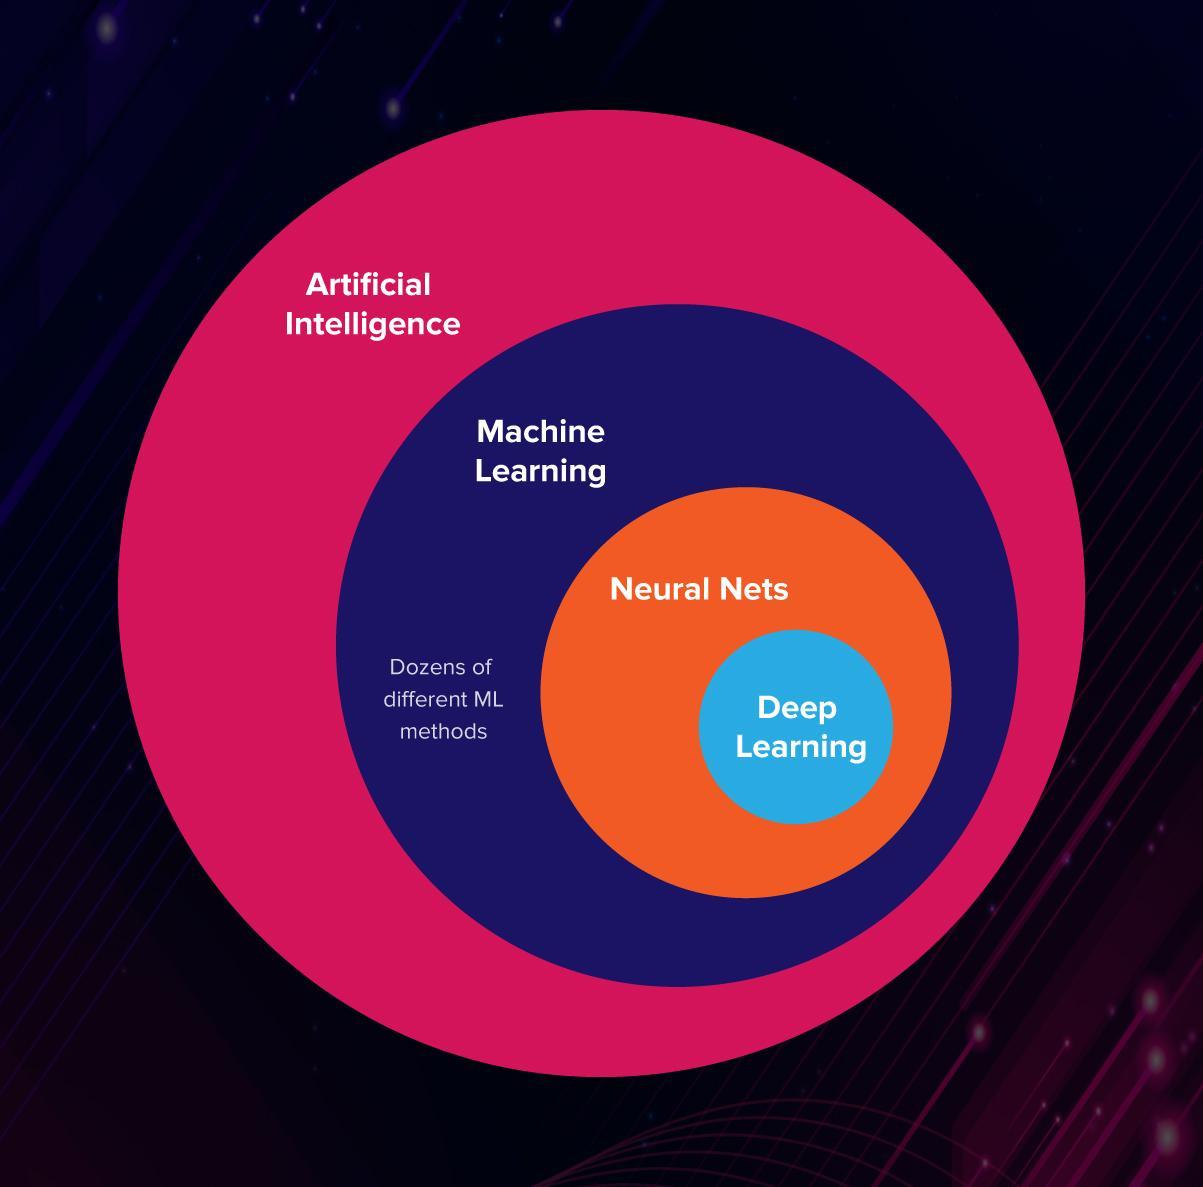
\includegraphics[width=\textwidth]{../manifest/ml-dl.jpg}
    \end{column}
\end{columns}
\end{frame}

% -----------------------------
% -------- SLAJD 25 ----------
% -----------------------------

\begin{frame}
\frametitle{Typy uczenia maszynowego}
    \begin{figure}
        \centering
        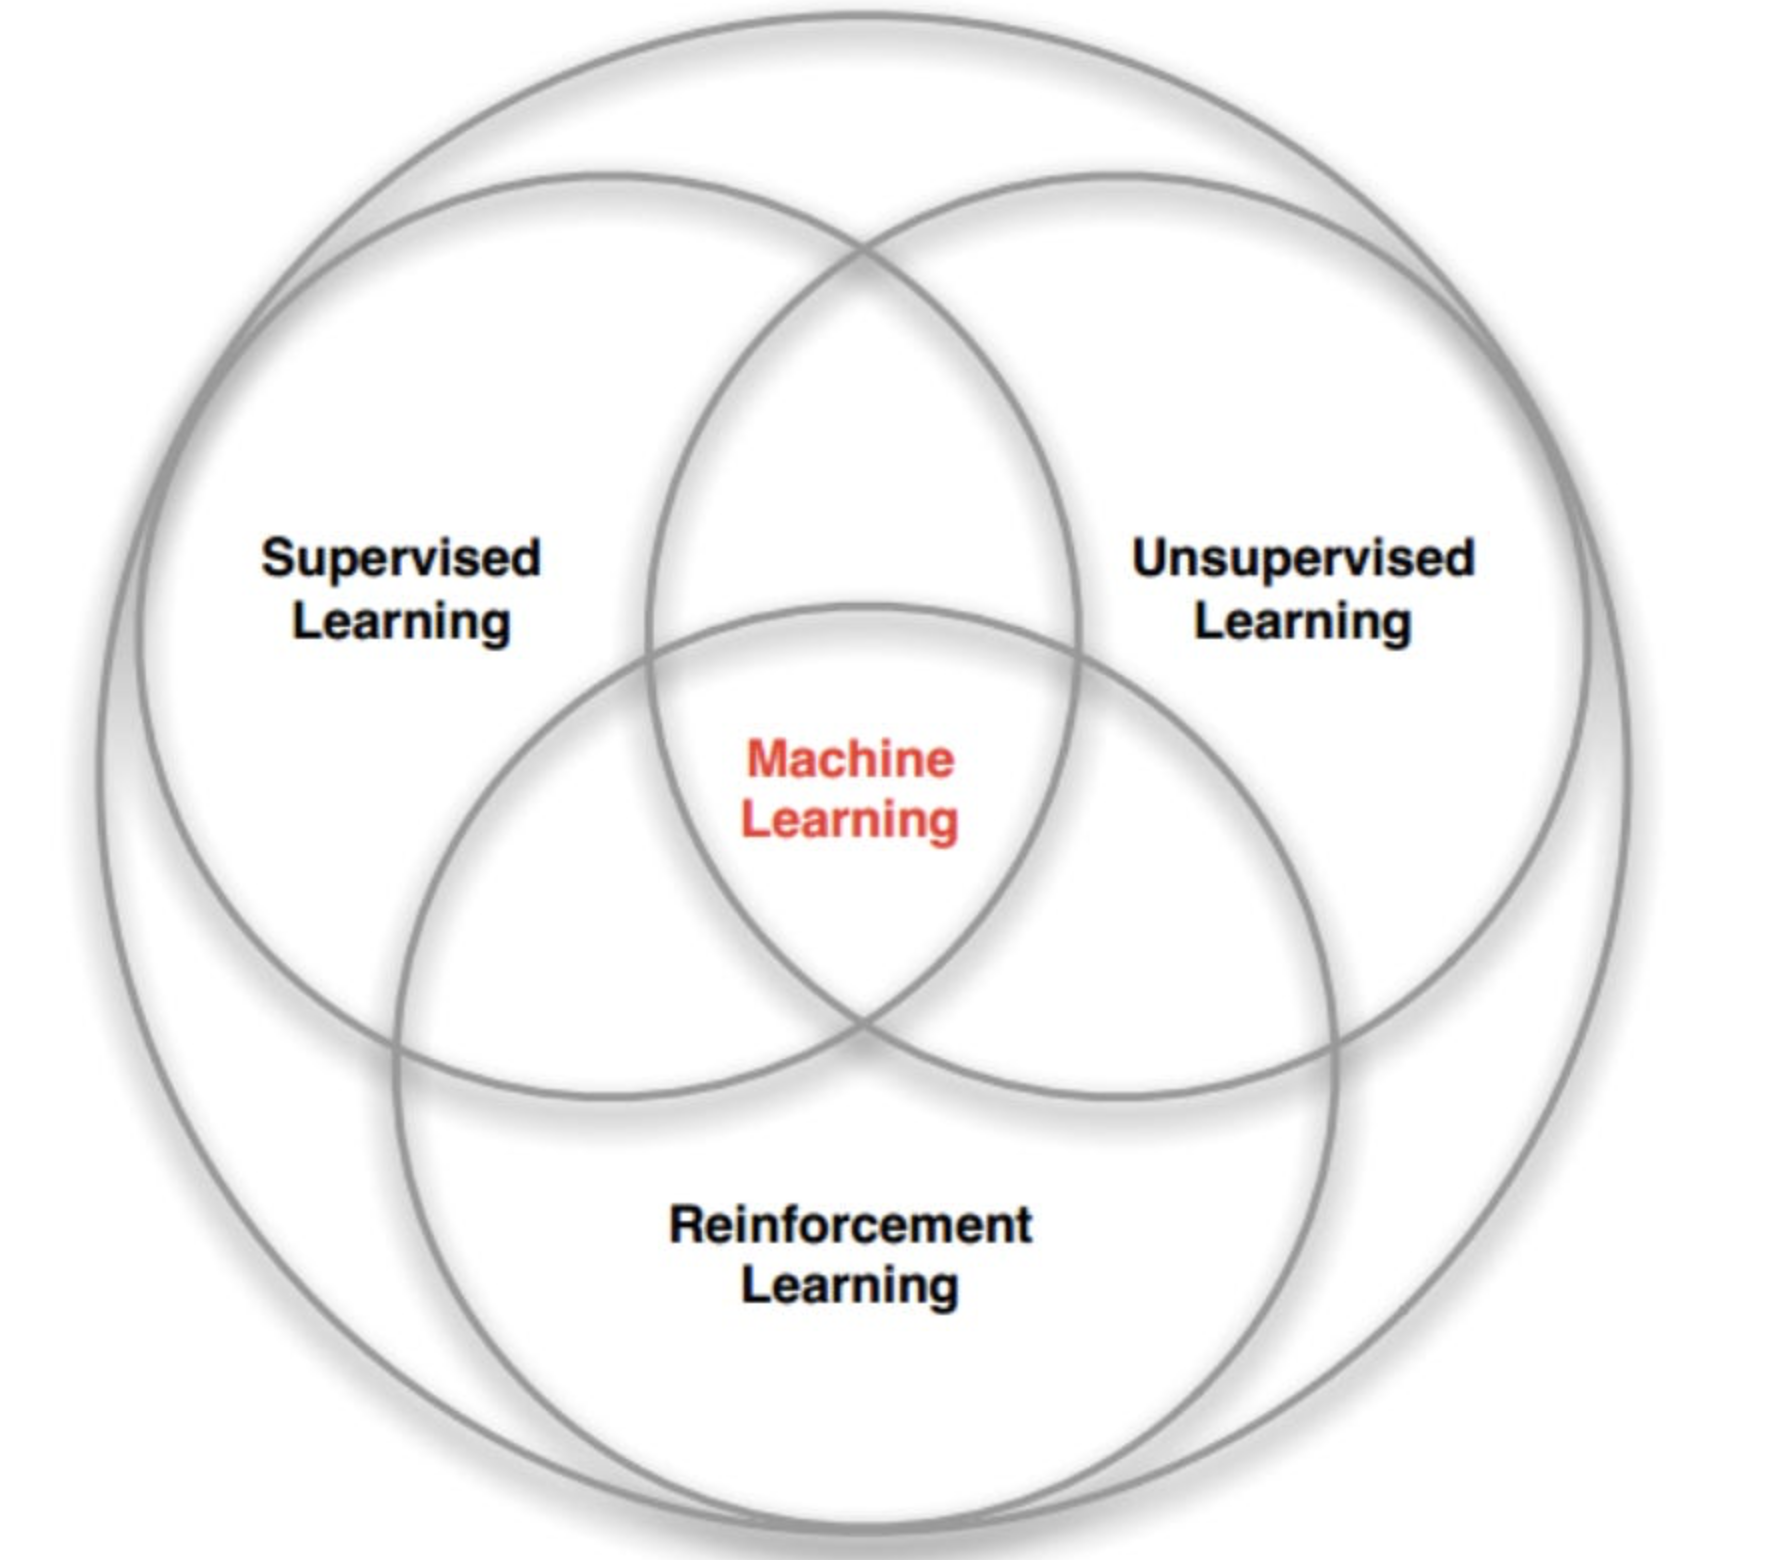
\includegraphics[width=\textwidth,height=0.7\textheight,keepaspectratio]{../manifest/ml-types.png}
    \end{figure}
\end{frame}


% -----------------------------
% -------- SLAJD 26 ----------
% -----------------------------

\begin{frame}
\frametitle{Typy uczenia maszynowego}

\begin{itemize}
    \item \textbf{\textcolor{red}{Uczenie nadzorowane (Supervised Learning):}} Model uczy się na podstawie \textbf{oznaczonych danych} i przewiduje wyniki na podstawie nowych danych. Przykłady to regresja i klasyfikacja.
    \item \textbf{Uczenie nienadzorowane (Unsupervised Learning):} Model uczy się wykrywać wzorce w danych, które nie są oznaczone. Przykłady to klasteryzacja i redukcja wymiarowości.
    \item \textbf{Uczenie przez wzmacnianie (Reinforcement Learning):} Model uczy się podejmować decyzje, wykonując akcje w środowisku, aby uzyskać jak największą nagrodę. \faHeart
\end{itemize}

\end{frame}

% -----------------------------
% -------- SLAJD 27 ----------
% -----------------------------

\begin{frame}
\frametitle{Co to jest głębokie uczenie?}

\begin{columns}
    \begin{column}{0.6\textwidth}
        \begin{itemize}
            \item Głębokie uczenie to część uczenia maszynowego oparta na \textbf{sieciach neuronowych}
            \item Umożliwia komputerom naukę z dużych ilości danych.
            \item Przykłady: Rozpoznawanie obrazów, generowanie tekstu, tłumaczenie języków.
        \end{itemize}
    \end{column}

    \begin{column}{0.4\textwidth}
        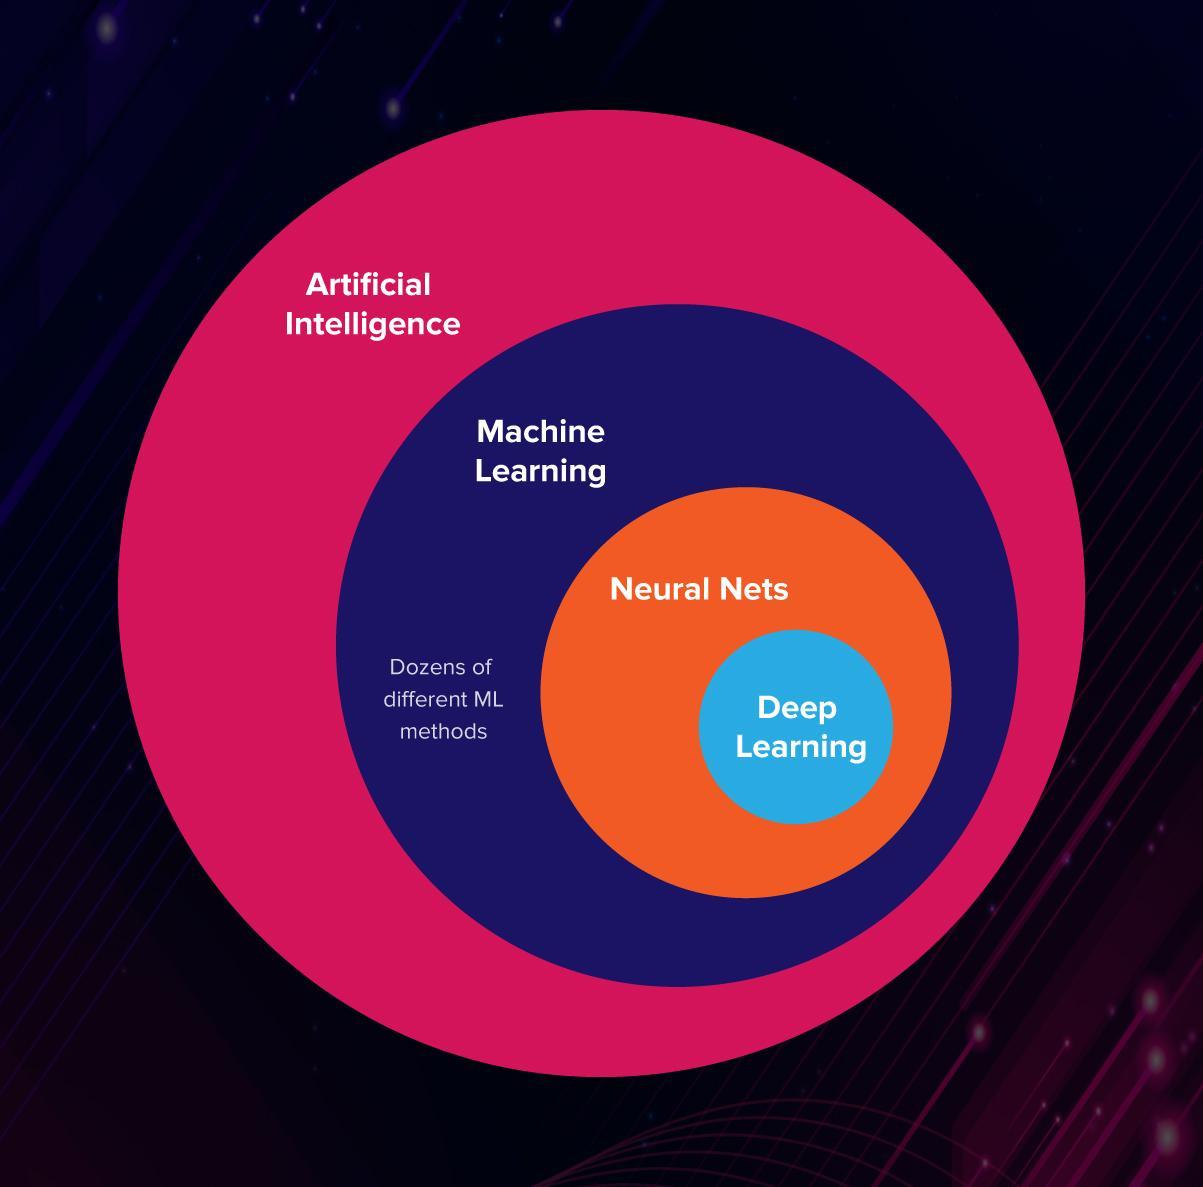
\includegraphics[width=\textwidth]{../manifest/ml-dl.jpg} % Wstaw ścieżkę do odpowiedniego obrazu
    \end{column}
\end{columns}
\end{frame}

% -----------------------------
% -------- SLAJD 28 -----------
% -----------------------------

\begin{frame}
\frametitle{Czy sieci neuronowe są naprawdę tak potężne?}

\begin{columns}
    \begin{column}{0.6\textwidth}
        \begin{itemize}
            \item Sieci neuronowe to potężne narzędzia, ale same w sobie \textbf{nie są "magiczne"}. To sposób, w jaki są używane w różnych architekturach i modelach, sprawia, że są skuteczne.
            \item Często słyszymy, że "sieci neuronowe osiągnęły coś niesamowitego", ale prawda jest taka, że to \textbf{\textcolor{red}{złożone modele i algorytmy, które wykorzystują sieci neuronowe}}, osiągają te wyniki.
        \end{itemize}
    \end{column}

    \begin{column}{0.4\textwidth}
        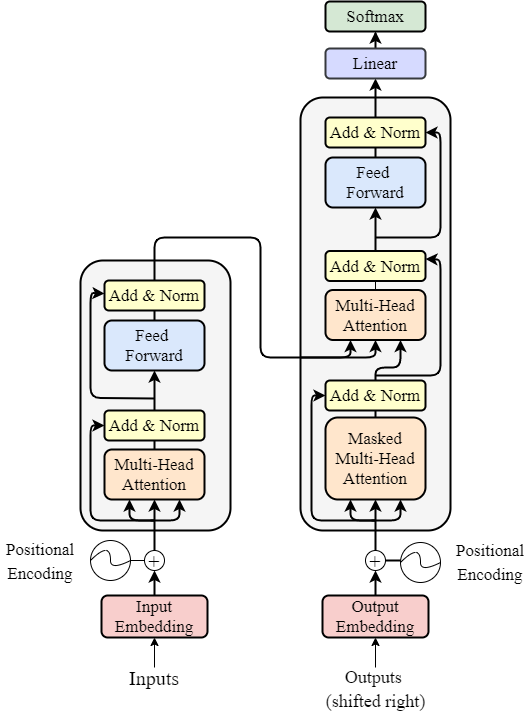
\includegraphics[width=\textwidth]{../manifest/transformer.png} % Wstaw ścieżkę do obrazu ilustrującego różne architektury
    \end{column}
\end{columns}
\end{frame}

% -----------------------------
% -------- SLAJD 29 -----------
% -----------------------------

\begin{frame}
\frametitle{Convolutional Neural Network}
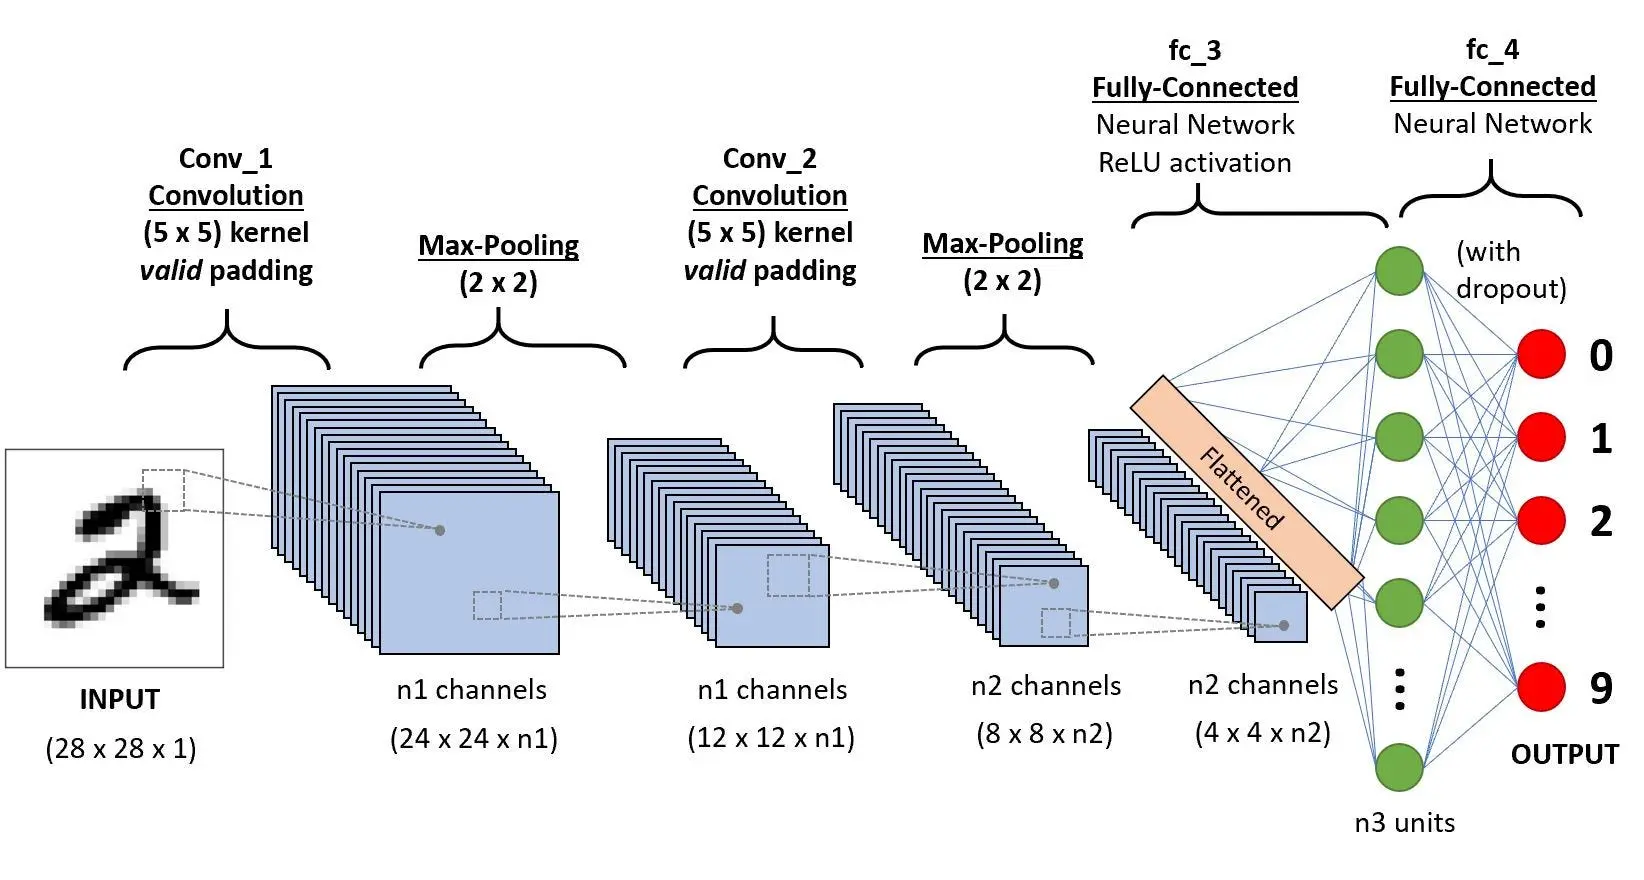
\includegraphics[width=\textwidth,height=0.8\textheight,keepaspectratio]{../manifest/deep-learning.png}
\end{frame}

% -----------------------------
% -------- SLAJD 30 -----------
% -----------------------------

\begin{frame}
\frametitle{You Only Look Once (YOLO)}
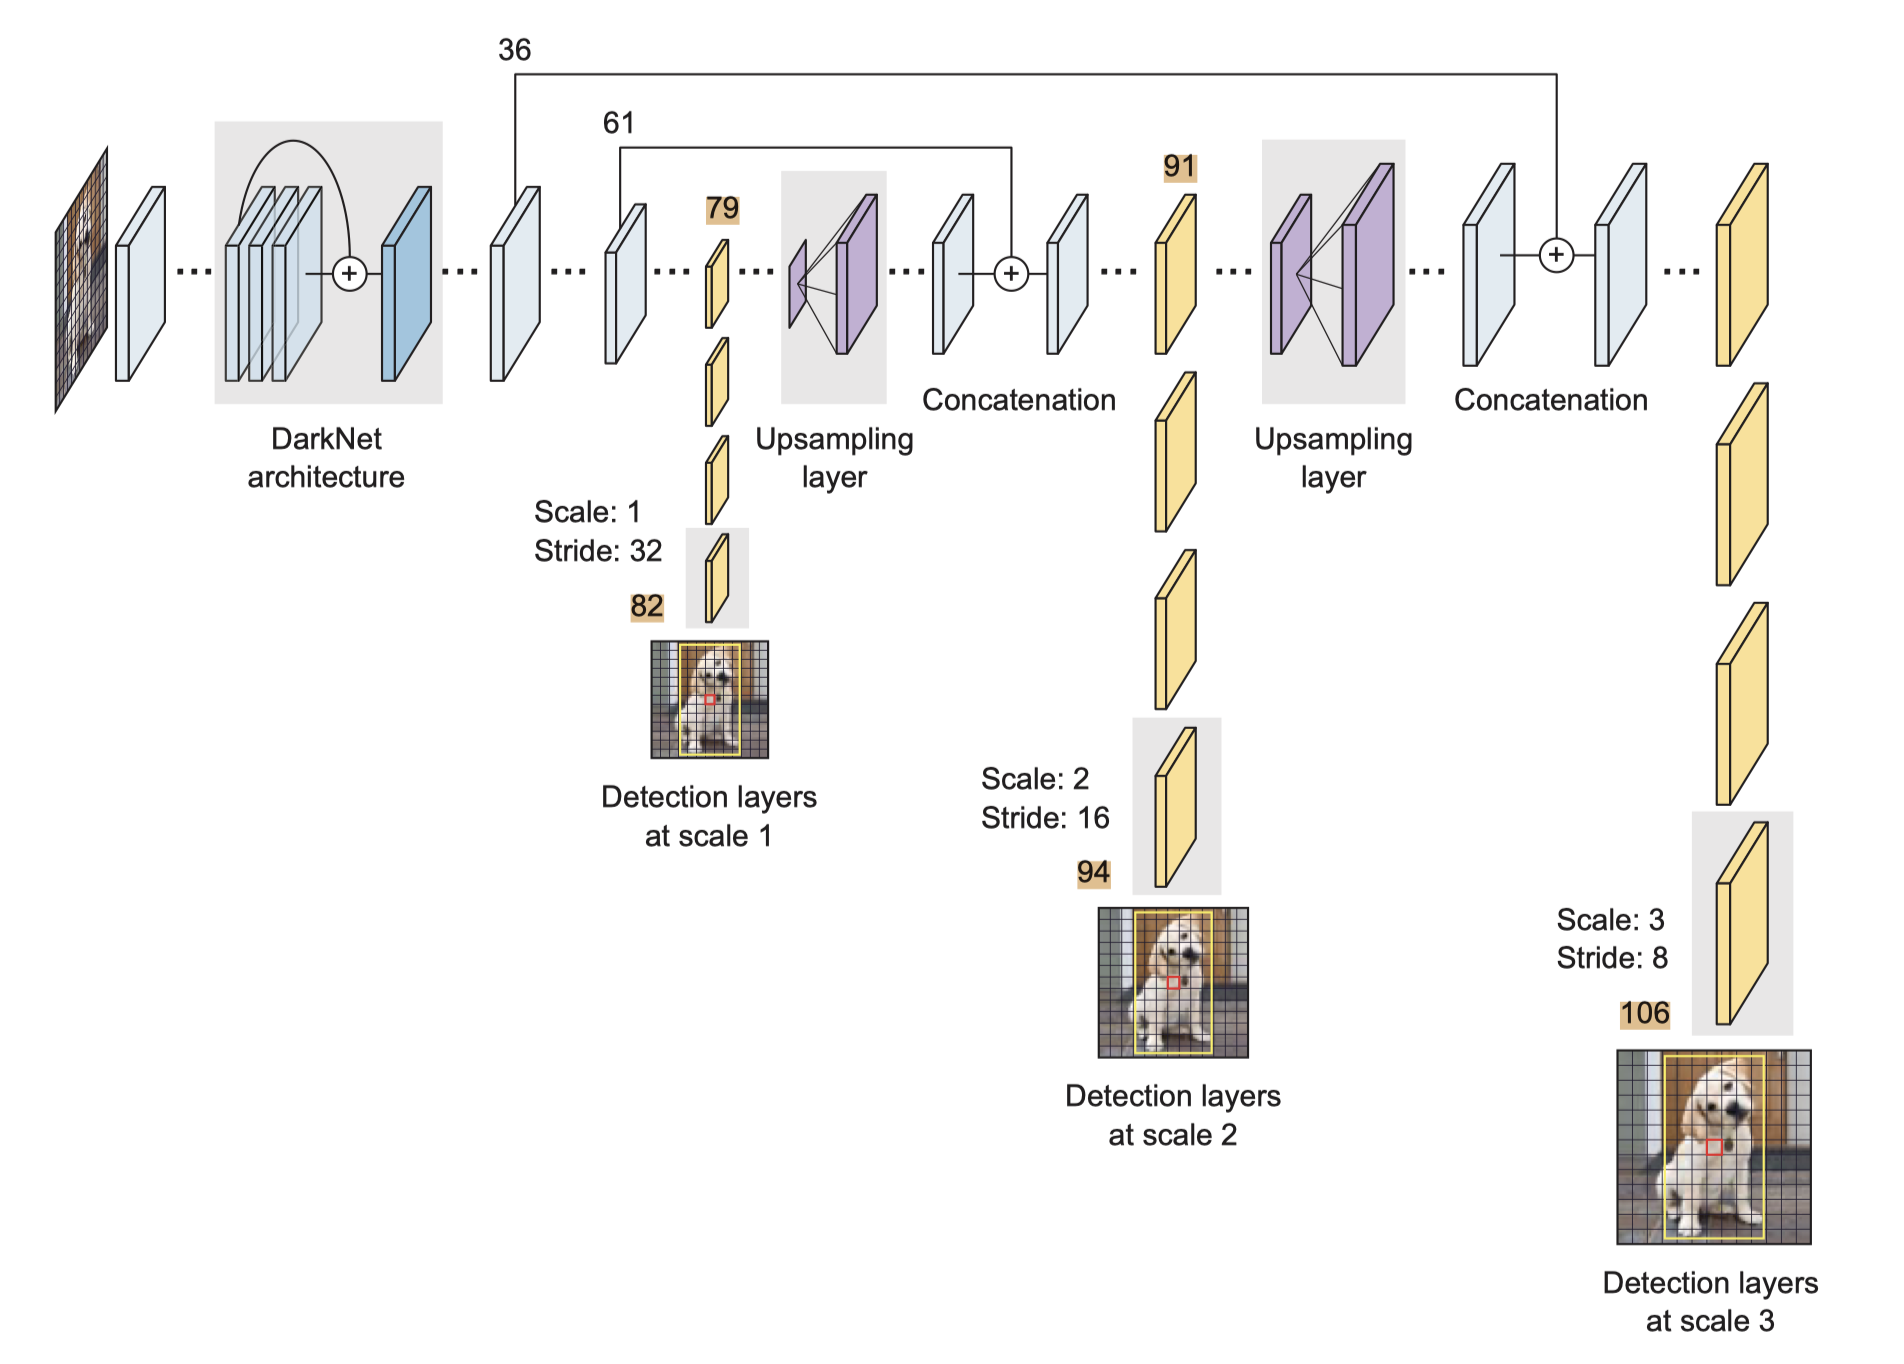
\includegraphics[width=\textwidth,height=0.8\textheight,keepaspectratio]{../manifest/yolo.png}
\end{frame}

% -----------------------------
% -------- SLAJD 31 -----------
% -----------------------------

\begin{frame}
\frametitle{}

\begin{center}
\Huge Jak działa uczenie nadzorowane?
\end{center}

\end{frame}

% -----------------------------
% -------- SLAJD 32 -----------
% -----------------------------

\begin{frame}
\frametitle{Nauczyciel w świecie maszyn: Uczenie Nadzorowane}

\begin{columns}
    \begin{column}{0.5\textwidth}
        \begin{itemize}
            \item \textbf{Nauczyciel:} W uczeniu nadzorowanym, "nauczyciel" (człowiek) pokazuje komputerowi, co ma się nauczyć, podając \textbf{przykłady danych i odpowiednich etykiet.}
            \item \textbf{Książka z odpowiedziami:} Podobnie jak w szkolnej książce z odpowiedziami, komputer otrzymuje zestaw pytań \textbf{wraz z odpowiedziami (etykiety)}, które pomagają mu się uczyć.
        \end{itemize}
    \end{column}

    \begin{column}{0.5\textwidth}
        \centering
        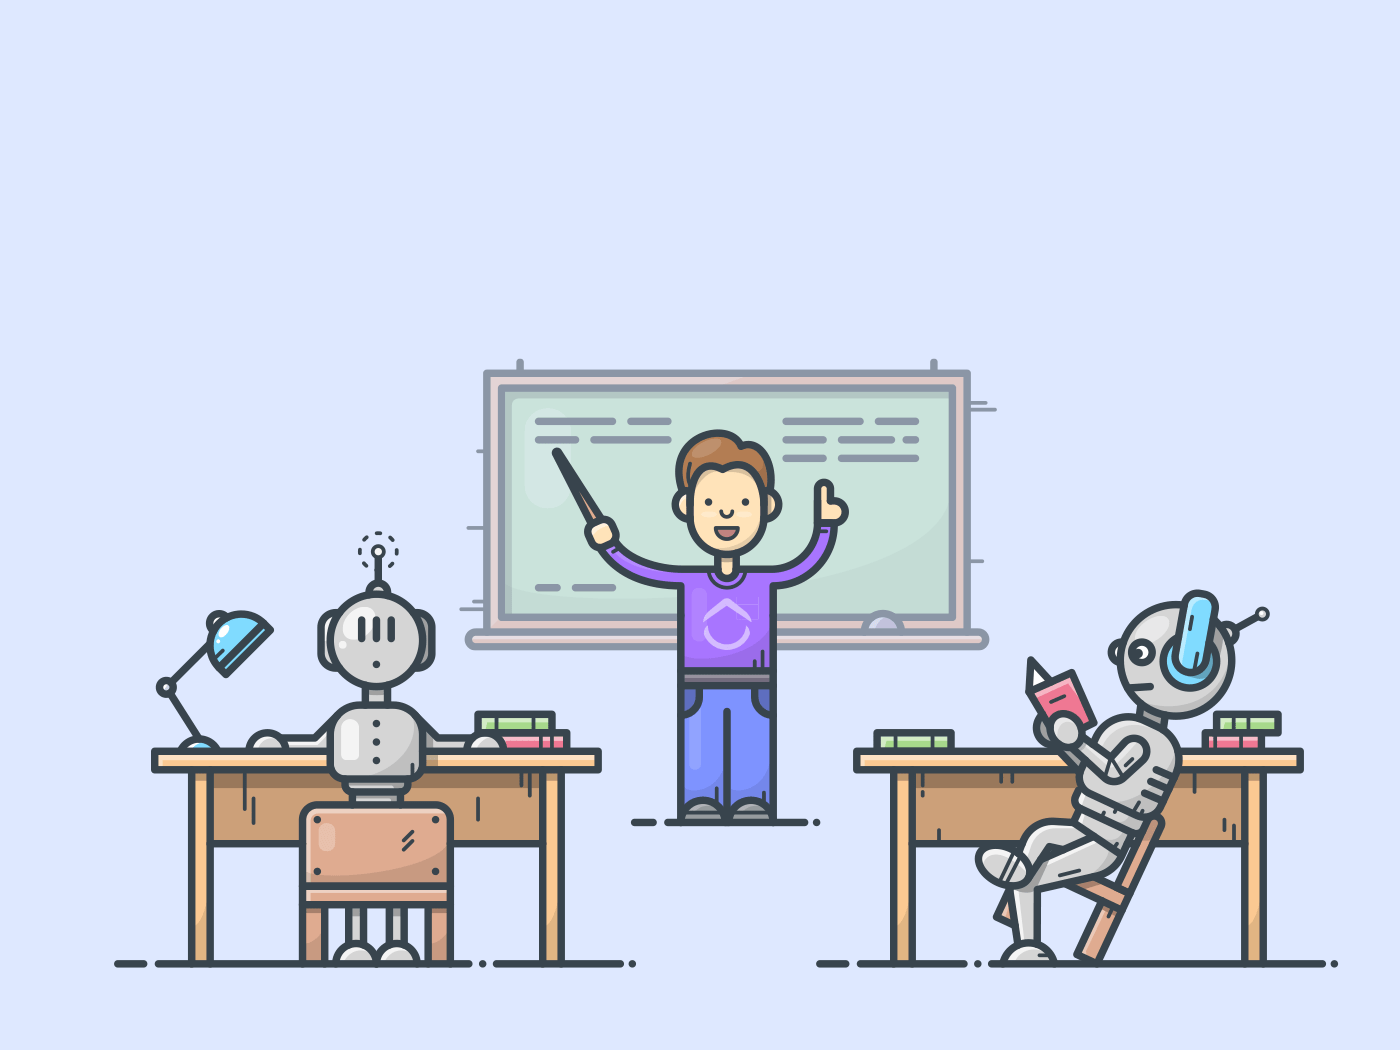
\includegraphics[width=\linewidth]{../manifest/sl-intuition.png}
    \end{column}
\end{columns}

\end{frame}

% -----------------------------
% -------- SLAJD 33 -----------
% -----------------------------

\begin{frame}
\frametitle{Problemy rozwiązywane przez uczenie nadzorowane}

\begin{columns}
    \begin{column}{0.5\textwidth}
        \begin{itemize}
            \item \textbf{Regresja:}
                \begin{itemize}
                    \item Przewidywanie ciągłych wartości.
                    \item Przykład: Estymacja ceny mieszkania na podstawie jego lokalizacji, rozmiaru i cech.
                \end{itemize}
        \end{itemize}
    \end{column}

    \begin{column}{0.5\textwidth}
        \begin{itemize}
            \item \textbf{Klasyfikacja:}
                \begin{itemize}
                    \item Przewidywanie dyskretnych etykiet.
                    \item Przykład: Rozpoznawanie kotków i piesków na zdjęciach.
                \end{itemize}
        \end{itemize}
    \end{column}
\end{columns}

\end{frame}

% -----------------------------
% -------- SLAJD 34 -----------
% -----------------------------

\begin{frame}
\frametitle{Klasyfikacja oraz regresja}
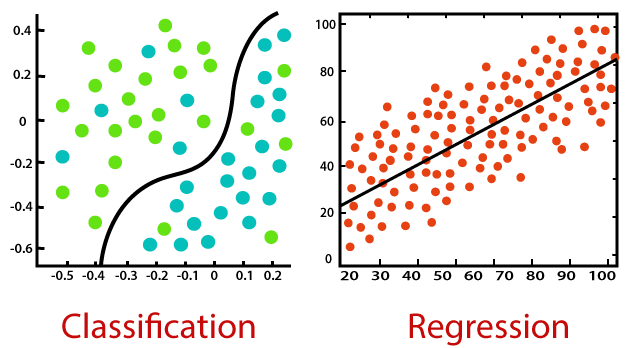
\includegraphics[width=\textwidth,height=0.8\textheight,keepaspectratio]{../manifest/regression-classification-1.png}
\end{frame}

% -----------------------------
% -------- SLAJD 31 -----------
% -----------------------------

\begin{frame}
\frametitle{Klasyfikacja oraz regresja}
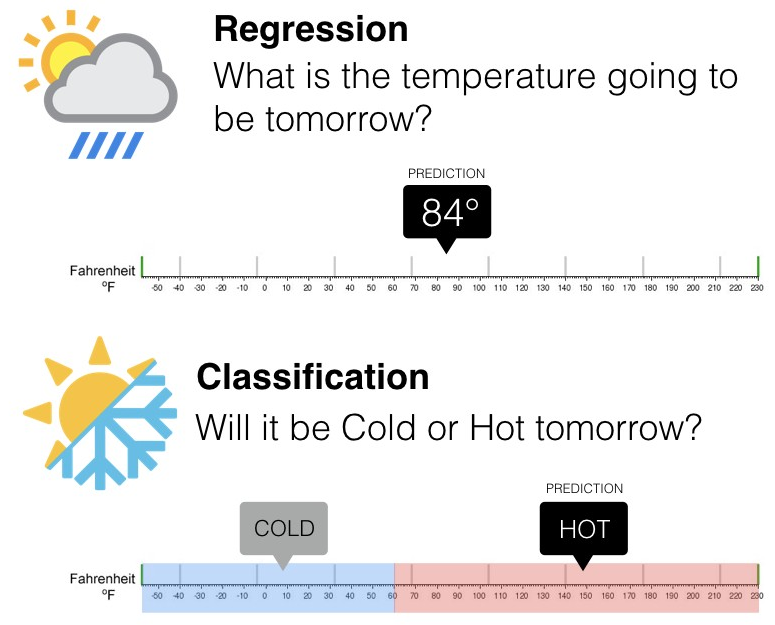
\includegraphics[width=\textwidth,height=0.8\textheight,keepaspectratio]{../manifest/regression-classification-2.png}
\end{frame}

% -----------------------------
% -------- SLAJD 35 -----------
% -----------------------------

\begin{frame}
\frametitle{Czym są dane oznaczone ?}

\begin{itemize}
    \item \textbf{Oznaczone odpowiedziami:} Dane oznaczone zawierają informacje wejściowe oraz odpowiadające im etykiety, które służą jako odpowiedzi.
    \item \textbf{Podstawa uczenia nadzorowanego:} Dzięki etykietom, model uczenia maszynowego może nauczyć się rozpoznawać wzorce i dokonywać przewidywań.
\end{itemize}

\end{frame}

% -----------------------------
% -------- SLAJD 36 -----------
% -----------------------------

\begin{frame}
\frametitle{Dane oznaczone}
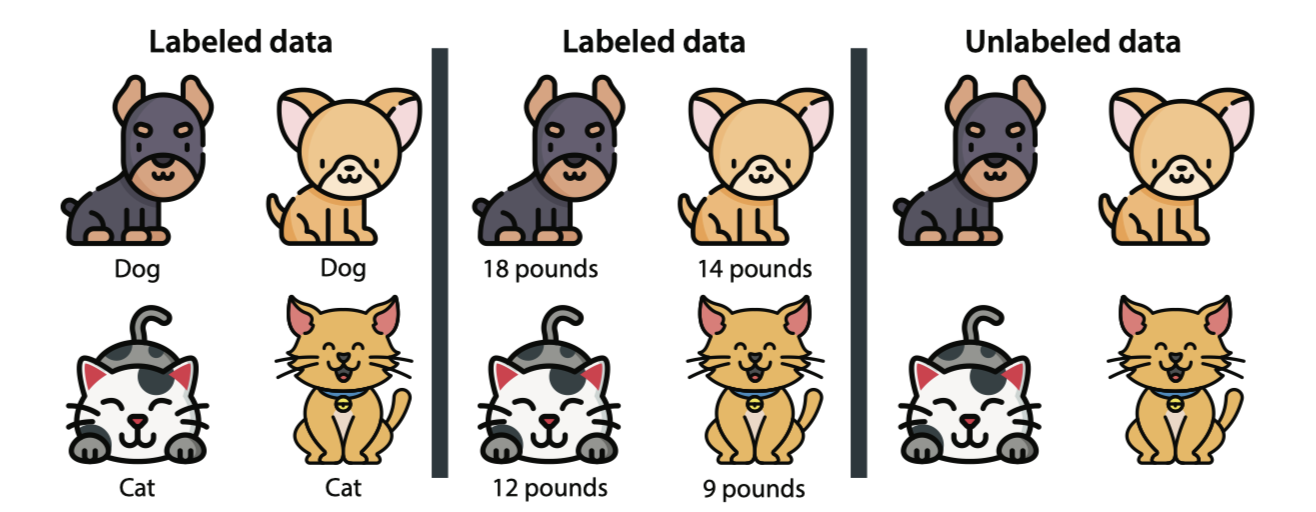
\includegraphics[width=\textwidth,height=0.8\textheight,keepaspectratio]{../manifest/labelled-data.png}
\end{frame}

% -----------------------------
% -------- SLAJD 37 -----------
% -----------------------------

\begin{frame}
\frametitle{Jak działa uczenie nadzorowane?}


\begin{columns}
    \begin{column}{0.4\textwidth}
        \begin{itemize}
            \item \textbf{Zapamiętanie:} Model uczy się na podstawie danych historycznych, które są "oznaczone" odpowiedziami.
            \item \textbf{Formułowanie:} Na podstawie tych danych, model "formułuje" zależności i wzorce.
            \item \textbf{Predykcja:} Używając nauczonych wzorców, model jest w stanie przewidywać przyszłe zdarzenia.
        \end{itemize}
    \end{column}

    \begin{column}{0.6\textwidth}
        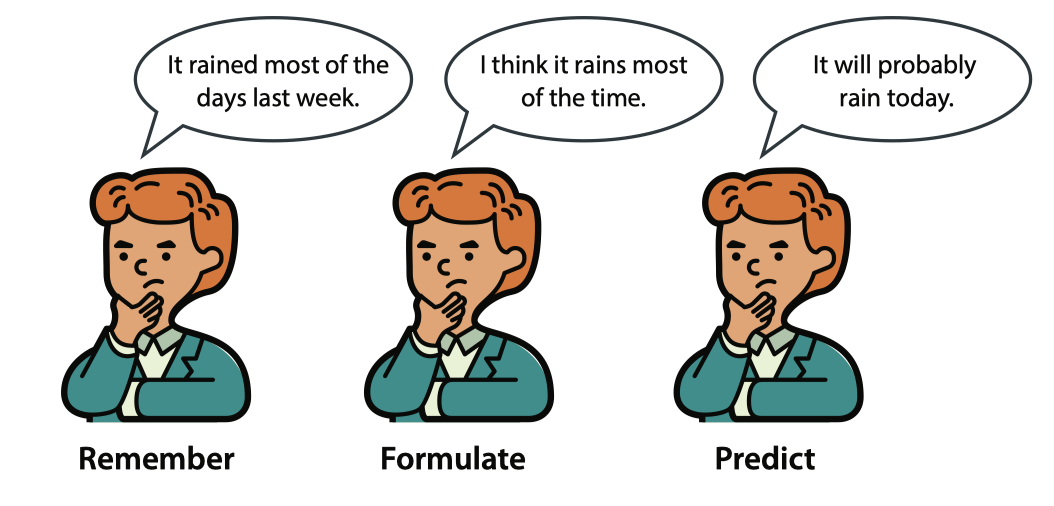
\includegraphics[width=\textwidth]{../manifest/r-f-p-1} 
    \end{column}
\end{columns}

\end{frame}

% -----------------------------
% -------- SLAJD 38 -----------
% -----------------------------

\begin{frame}
\frametitle{Klasyfikator piesków i kotków}
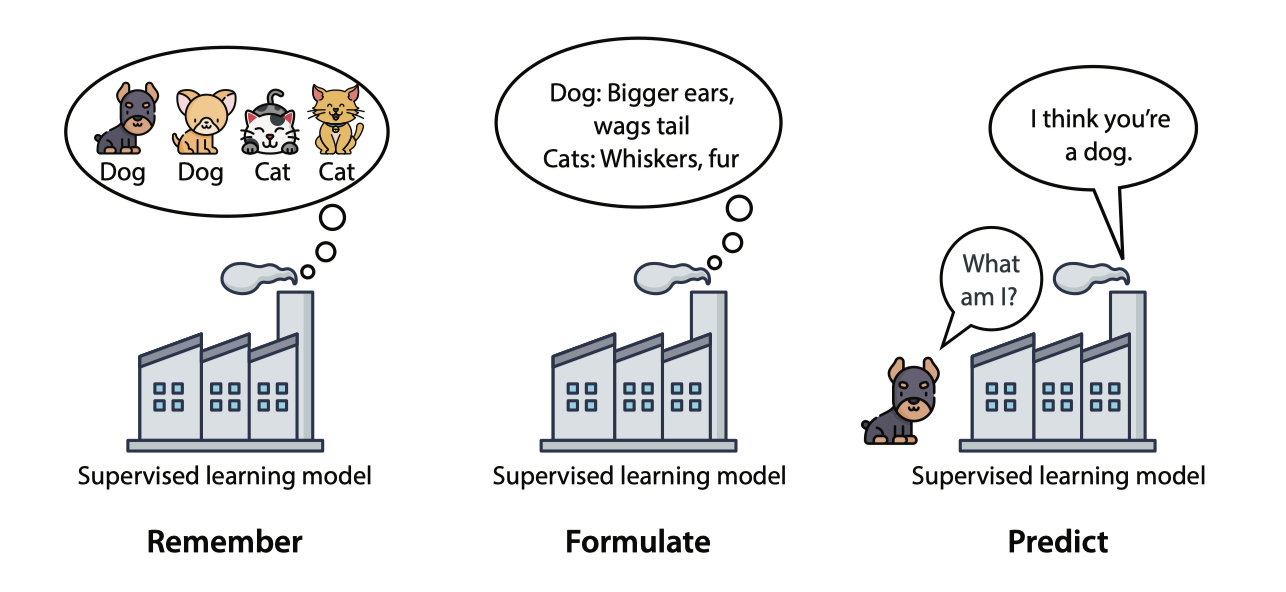
\includegraphics[width=\textwidth,height=0.8\textheight,keepaspectratio]{../manifest/r-f-p-2.png}
\end{frame}

% -----------------------------
% -------- SLAJD 39 -----------
% -----------------------------

\begin{frame}
\frametitle{Klasyfikator piesków i kotków}
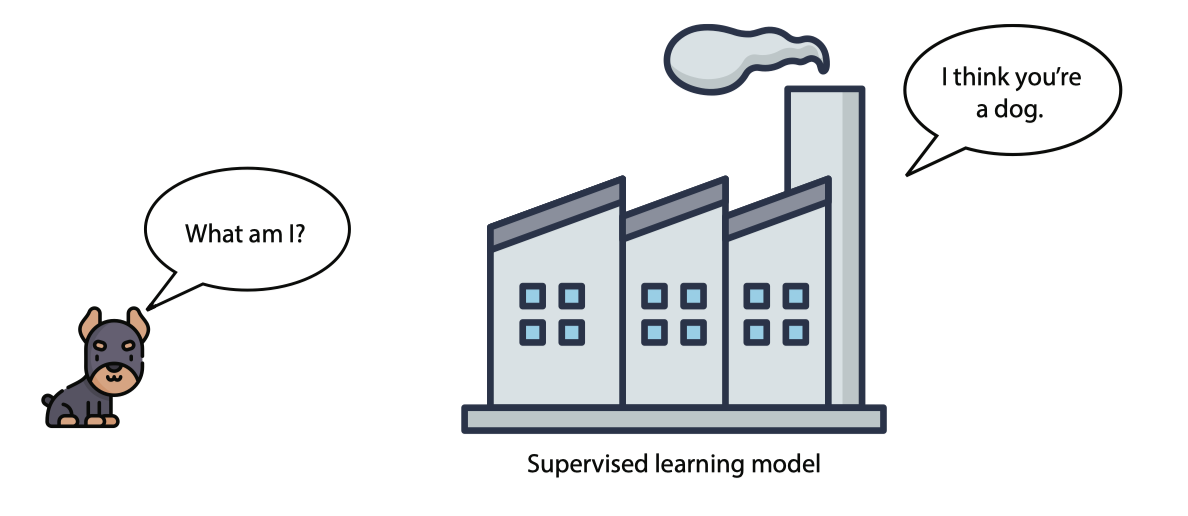
\includegraphics[width=\textwidth,height=0.8\textheight,keepaspectratio]{../manifest/r-f-p-3.png}
\end{frame}

% -----------------------------
% -------- SLAJD 40 -----------
% -----------------------------

\begin{frame}
\frametitle{Regresja ceny mieszkań (R-F-P)}
\begin{figure}
    \centering
    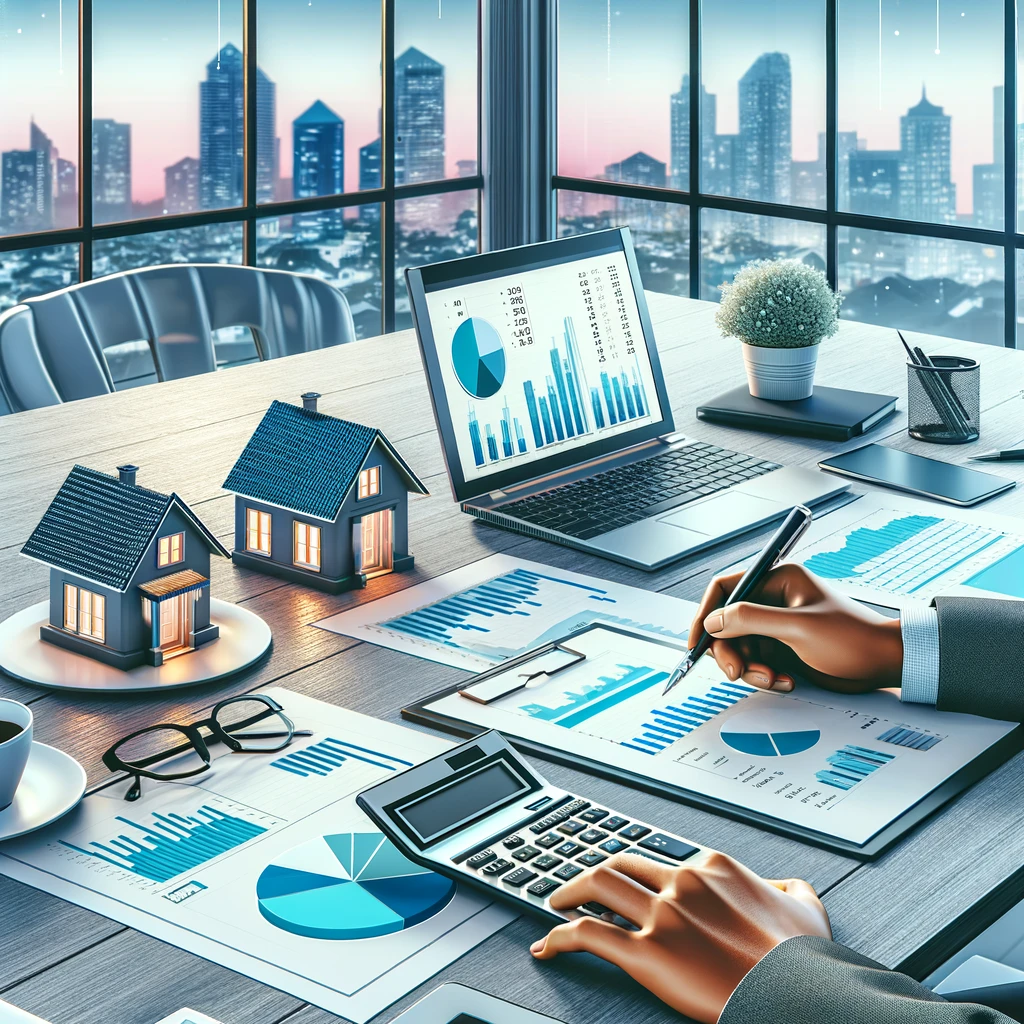
\includegraphics[width=\textwidth,height=0.7\textheight,keepaspectratio]{../manifest/real-estate.png}
\end{figure}
\end{frame}

% -----------------------------
% -------- SLAJD 41 -----------
% -----------------------------

\begin{frame}
\frametitle{Cena mieszkania w.r.t ilości pokoi}
\begin{figure}
    \centering
    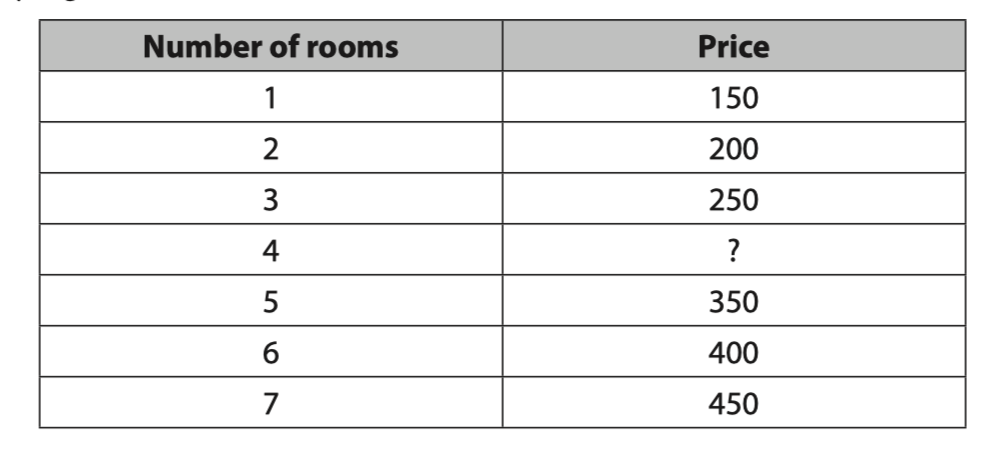
\includegraphics[width=\textwidth,height=0.7\textheight,keepaspectratio]{../manifest/estate-data-raw.png}
\end{figure}
\end{frame}

% -----------------------------
% -------- SLAJD 42 -----------
% -----------------------------

\begin{frame}
\frametitle{Step 1. R-emember (Zapamiętywanie danych oraz etykiet)}
\begin{figure}
    \centering
    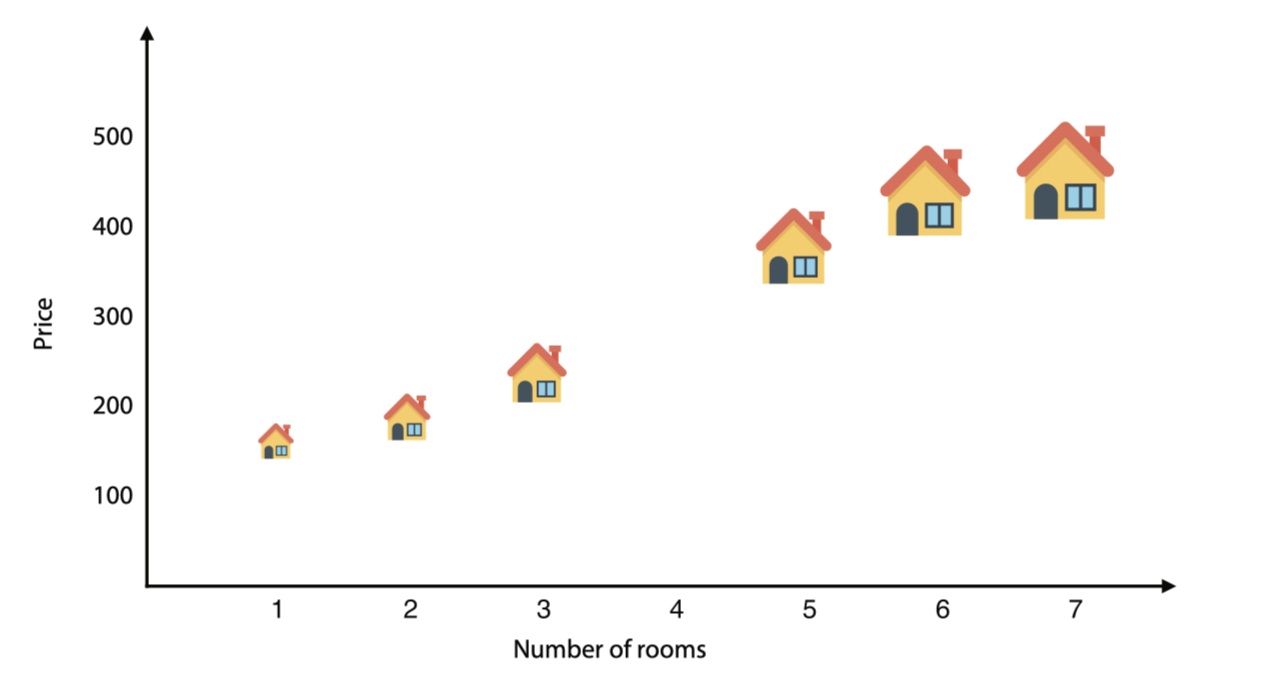
\includegraphics[width=\textwidth,height=0.7\textheight,keepaspectratio]{../manifest/estate-remember.png}
\end{figure}
\end{frame}

% -----------------------------
% -------- SLAJD 43 -----------
% -----------------------------

\begin{frame}
\frametitle{Step 2. F-ormulate (Formułowanie Zasad)}
\begin{figure}
    \centering
    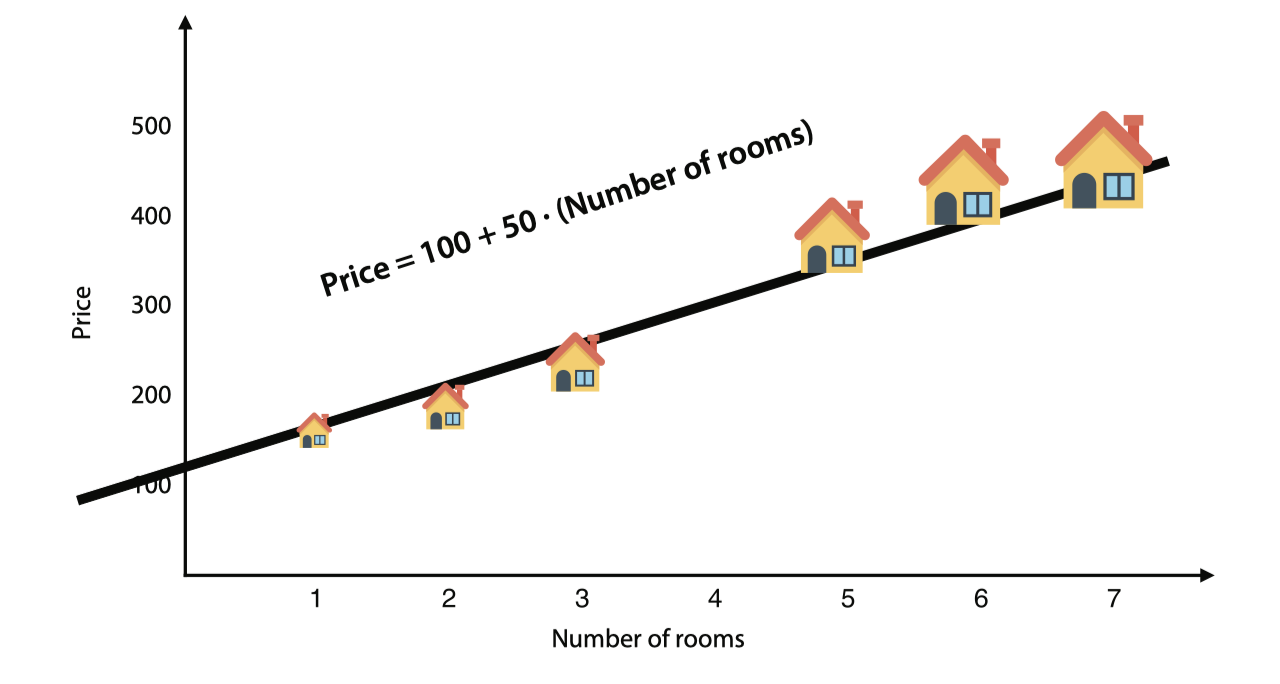
\includegraphics[width=\textwidth,height=0.7\textheight,keepaspectratio]{../manifest/estate-formulate.png}
\end{figure}
\end{frame}

% -----------------------------
% -------- SLAJD 44 -----------
% -----------------------------

\begin{frame}
\frametitle{Cena mieszkania w.r.t ilości pokoi}
\begin{figure}
    \centering
    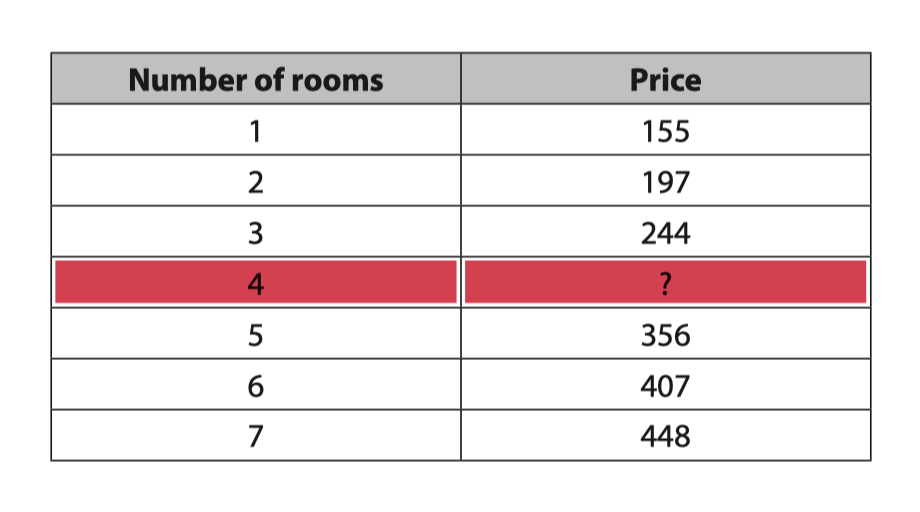
\includegraphics[width=\textwidth,height=0.7\textheight,keepaspectratio]{../manifest/estate-data.png}
\end{figure}
\end{frame}

% -----------------------------
% -------- SLAJD 45 -----------
% -----------------------------

\begin{frame}
\frametitle{Step 3. P-redict (Predykcja etykiet których nie znamy)}

\begin{columns}
    \begin{column}{0.5\textwidth}
        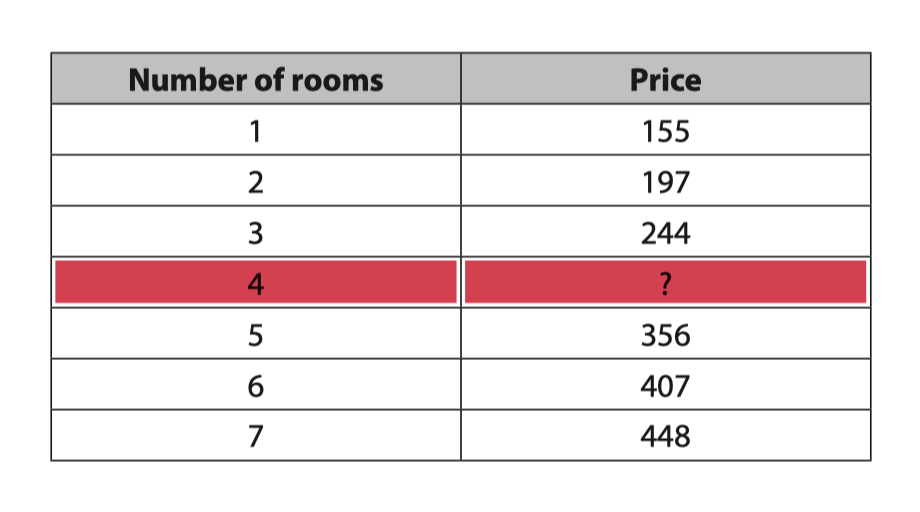
\includegraphics[width=\linewidth]{../manifest/estate-data.png} 
        \centering
    \end{column}
    \begin{column}{0.5\textwidth}
        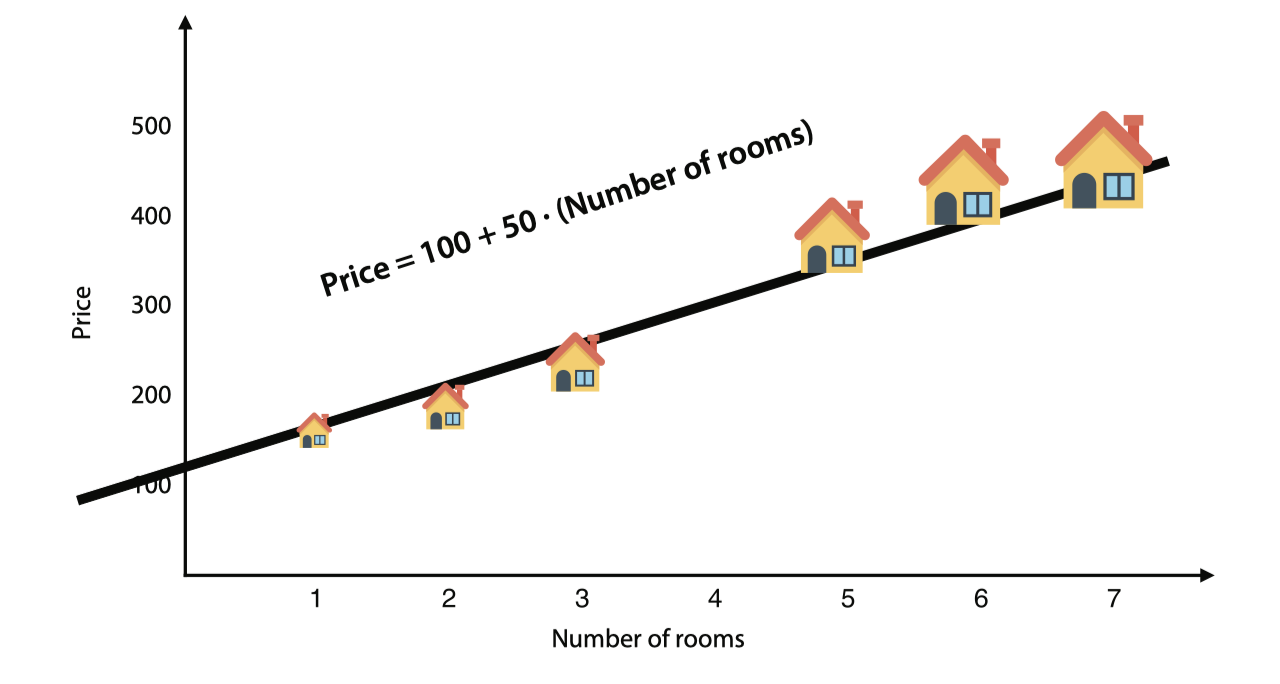
\includegraphics[width=\linewidth]{../manifest/estate-formulate}
        \centering
    \end{column}
\end{columns}

\end{frame}

% -----------------------------
% -------- SLAJD 46 -----------
% -----------------------------

\begin{frame}
\frametitle{Step 3. P-redict (Predykcja etykiet którcyh nie znamy)}
\begin{figure}
    \centering
    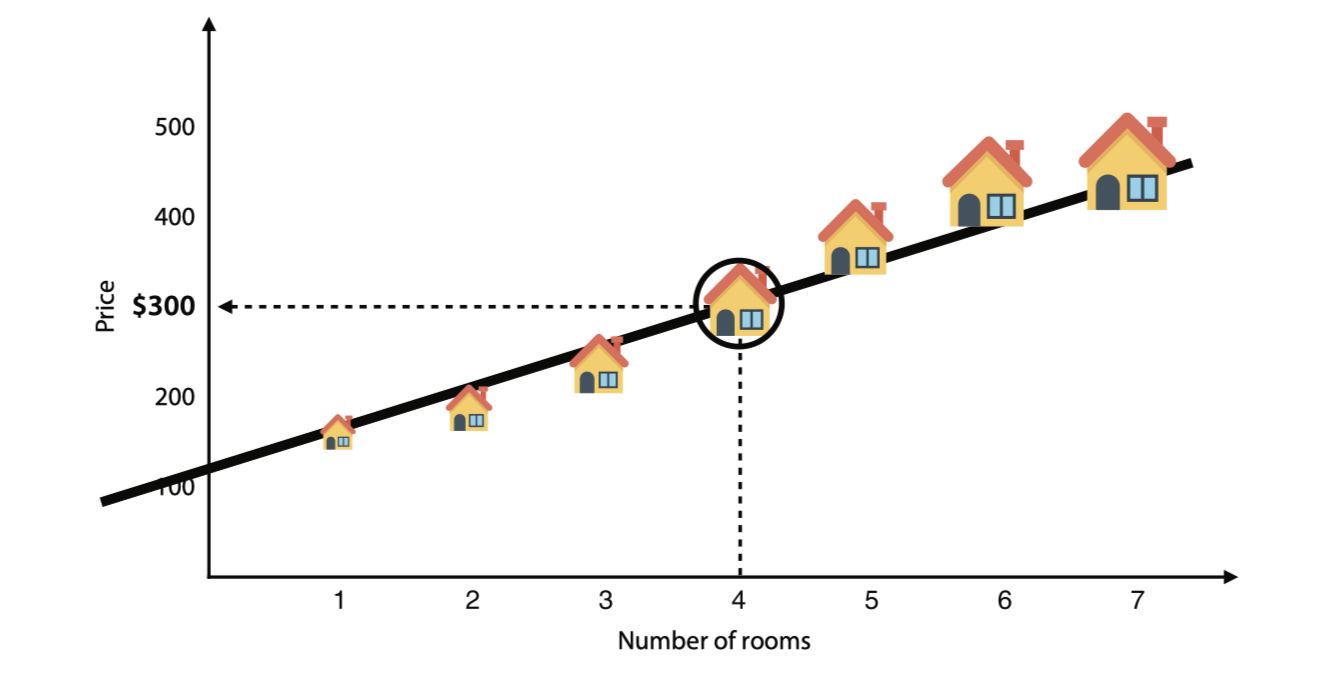
\includegraphics[width=\textwidth,height=0.7\textheight,keepaspectratio]{../manifest/estate-predict.png}
\end{figure}
\end{frame}

% -----------------------------
% -------- SLAJD 47 -----------
% -----------------------------

\begin{frame}
\frametitle{Perceptron: równanie liniowe i funkcja aktywacji}

\begin{columns}
    \begin{column}{0.4\textwidth}
        \begin{itemize}
            \item Perceptron Składa się z \textbf{równania liniowego}, które sumuje wejścia pomnożone przez ich wagi, 
            \item \textbf{\textcolor{red}{\( \sum_{i=1}^{n} w_i x_i + b \)}}
            \item gdzie \( w_i \) to waga i-tego wejścia \( x_i \), a \( b \) to wyraz wolny (bias).
        \end{itemize}
    \end{column}

    \begin{column}{0.6\textwidth}
        \centering
        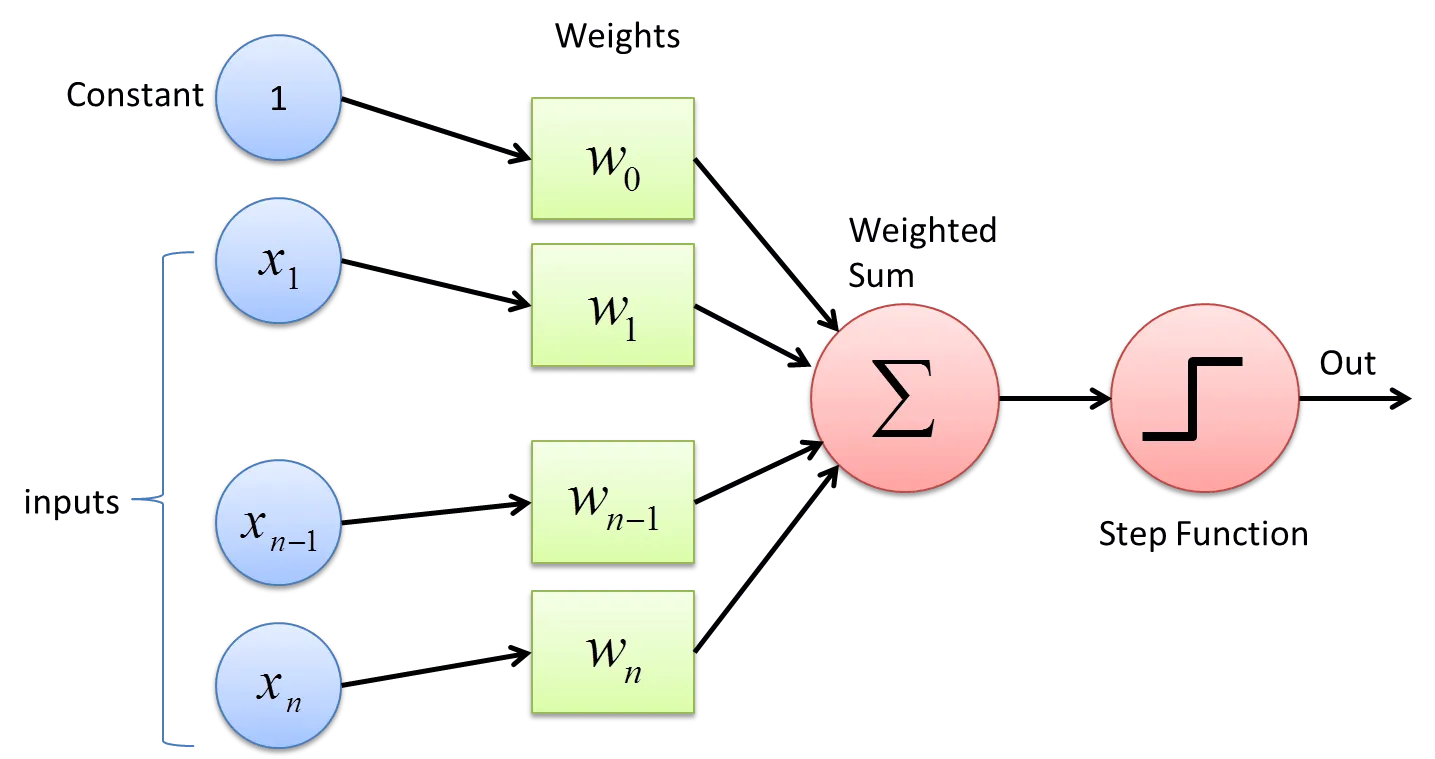
\includegraphics[width=\textwidth]{../manifest/perceptron.png} % Wstaw ścieżkę do obrazu przedstawiającego perceptron
    \end{column}
\end{columns}

\end{frame}

% -----------------------------
% -------- SLAJD 48 -----------
% -----------------------------

\begin{frame}
\frametitle{Równanie bez aktywacji}
\begin{figure}
    \centering
    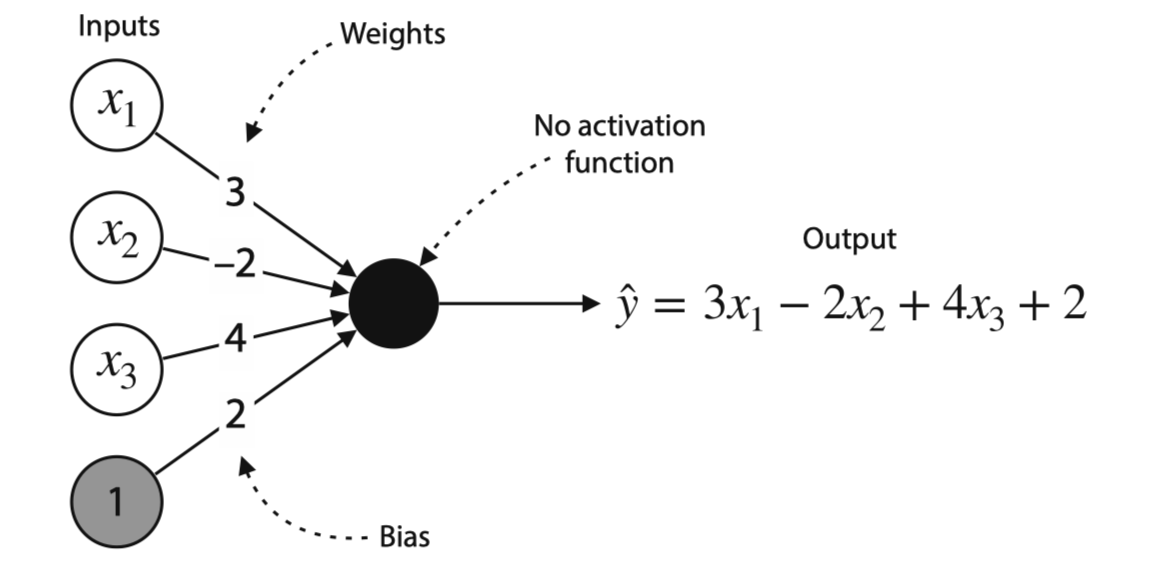
\includegraphics[width=\textwidth,height=0.7\textheight,keepaspectratio]{../manifest/no-activation.png}
\end{figure}
\end{frame}

% -----------------------------
% -------- SLAJD 49 -----------
% -----------------------------

\begin{frame}
\frametitle{Dane które można separować liniowo}
\begin{figure}
    \centering
    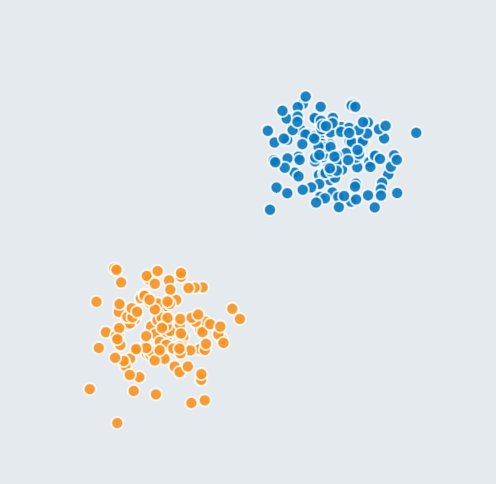
\includegraphics[width=\textwidth,height=0.7\textheight,keepaspectratio]{../manifest/linear-data.png}
\end{figure}
\end{frame}

% -----------------------------
% -------- SLAJD 50 -----------
% -----------------------------

\begin{frame}
\frametitle{Funkcja liniowa to za mało}
\begin{figure}
    \centering
    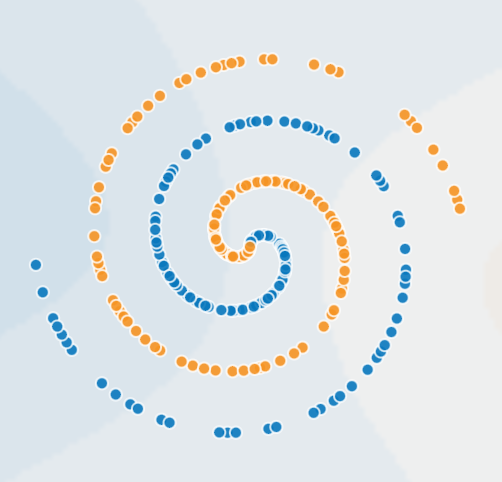
\includegraphics[width=\textwidth,height=0.7\textheight,keepaspectratio]{../manifest/non-linear-data.png}
\end{figure}
\end{frame}

% -----------------------------
% -------- SLAJD 51 -----------
% -----------------------------

\begin{frame}
\frametitle{Równanie z aktywacją}
\begin{figure}
    \centering
    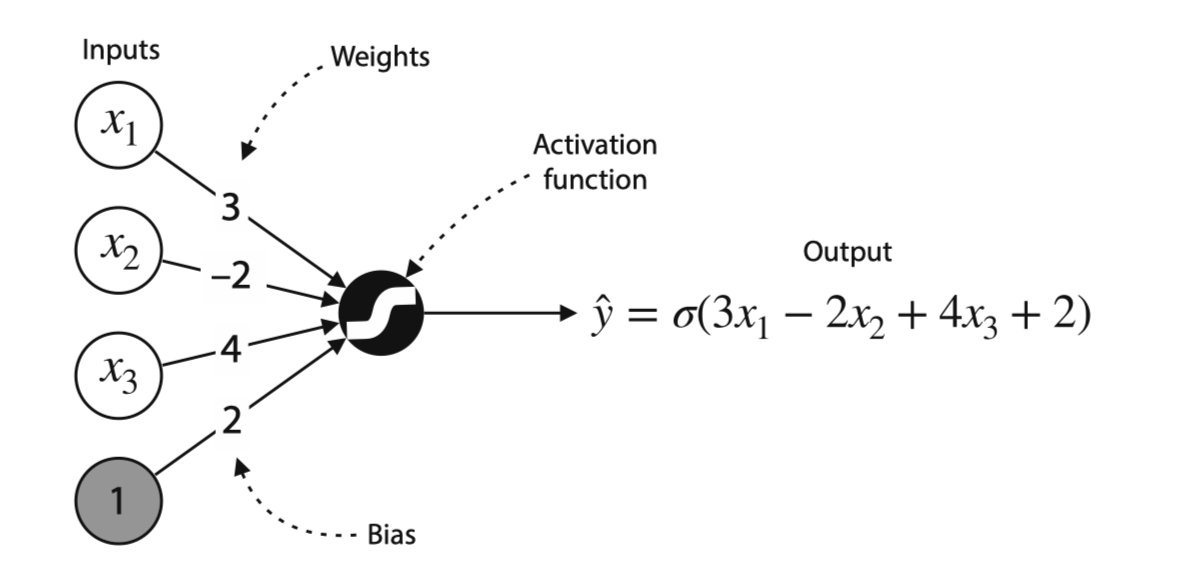
\includegraphics[width=\textwidth,height=0.7\textheight,keepaspectratio]{../manifest/activation.png}
\end{figure}
\end{frame}

% -----------------------------
% -------- SLAJD 52 -----------
% -----------------------------

\begin{frame}
\frametitle{Przewaga aktywacji}
\begin{figure}
    \centering
    \includegraphics[width=\textwidth,height=0.7\textheight,keepaspectratio]{../manifest/step-non-linear.png}
\end{figure}
\end{frame}

% -----------------------------
% -------- SLAJD 53 -----------
% -----------------------------

\begin{frame}
\frametitle{Nieliniowe wzorce}
\begin{figure}
    \centering
    \includegraphics[width=\textwidth,height=0.7\textheight,keepaspectratio]{../manifest/non-linear.png}
\end{figure}
\end{frame}

% -----------------------------
% -------- SLAJD 54 -----------
% -----------------------------

\begin{frame}
\frametitle{Sieć neuronowa z aktywacją}
\begin{figure}
    \centering
    \includegraphics[width=\textwidth,height=0.7\textheight,keepaspectratio]{../manifest/separation.png}
\end{figure}
\end{frame}

% -----------------------------
% -------- SLAJD 55 -----------
% -----------------------------

\begin{frame}
\frametitle{}

\begin{center}
\Huge Co w przypadku gdy model się pomyli?
\end{center}

\end{frame}

% -----------------------------
% -------- SLAJD 56 -----------
% -----------------------------

\begin{frame}
\frametitle{Uczenie modelu poprawnego zachowania}
    \centering
    \includegraphics[width=\textwidth,height=0.8\textheight,keepaspectratio]{../manifest/bad-model.png}
\end{frame}

% -----------------------------
% -------- SLAJD 57 -----------
% -----------------------------

\begin{frame}
\frametitle{Dobre oraz złe zachowanie - regresja ceny mieszkań}
    \centering
    \includegraphics[width=\textwidth,height=0.8\textheight,keepaspectratio]{../manifest/errors.png}
\end{frame}


% -----------------------------
% -------- SLAJD 58 -----------
% -----------------------------

\begin{frame}
\frametitle{Funkcja straty L1 (MAE)}

\begin{columns}
    \begin{column}{0.4\textwidth}
        \begin{itemize}
            \item \textbf{Definicja:} L1, czyli błąd bezwzględny średni (MAE), 
            \item mierzy średnią wartość bezwzględnych różnic między przewidywaniami a rzeczywistymi wartościami.
        \end{itemize}
    \end{column}
    \begin{column}{0.6\textwidth}
        \includegraphics[width=\linewidth]{../manifest/l1.png}
    \end{column}
\end{columns}

\end{frame}

% -----------------------------
% -------- SLAJD 59 -----------
% -----------------------------

\begin{frame}
\frametitle{Funkcja straty L2 (MSE)}

\begin{columns}
    \begin{column}{0.4\textwidth}
        \begin{itemize}
            \item \textbf{Definicja:} L2, czyli błąd średniokwadratowy (MSE),
            \item mierzy średnią wartość kwadratów różnic między przewidywaniami a rzeczywistymi wartościami.
        \end{itemize}
    \end{column}
    \begin{column}{0.6\textwidth}
        \includegraphics[width=\linewidth]{../manifest/l2.png}
    \end{column}
\end{columns}

\end{frame}

% -----------------------------
% -------- SLAJD 60 -----------
% -----------------------------

\begin{frame}
\frametitle{Co mówi błąd do modelu}
    \centering
    \includegraphics[width=\textwidth,height=0.8\textheight,keepaspectratio]{../manifest/points-move.png}
\end{frame}

% -----------------------------
% -------- SLAJD 61 -----------
% -----------------------------

\begin{frame}
\frametitle{Minimalizacja błędu}
    \centering
    \includegraphics[width=\textwidth,height=0.8\textheight,keepaspectratio]{../manifest/error-optim.png}
\end{frame}

% -----------------------------
% -------- SLAJD 62 -----------
% -----------------------------

% -----------------------------
% -------- PODSUMOWANIE -------
% -----------------------------

\begin{frame}
\frametitle{Podsumowanie: Uczenie maszynowe i jego aspekty}

\begin{itemize}
    \item Uczenie maszynowe to dziedzina sztucznej inteligencji skoncentrowana na rozwijaniu algorytmów, które mogą uczyć się z danych i dokonywać prognoz lub decyzji bez jawnego programowania.
    \item Uczenie nadzorowane, jedna z głównych kategorii uczenia maszynowego, zajmuje się problemami regresji i klasyfikacji poprzez analizowanie danych etykietowanych.
    \item Sieci neuronowe wykorzystują funkcje aktywacji do wprowadzania nieliniowości w procesie uczenia, co pozwala na modelowanie skomplikowanych wzorców w danych.
\end{itemize}

\end{frame}

% -----------------------------
% -------- AGENDA -------------
% -----------------------------

\begin{frame}
\frametitle{Agenda}
\begin{enumerate}
    \item \color{gray}Historia i rozwój AI
    \item \color{gray}Przerwa
    \item \color{gray}Podstawy uczenia maszynowego i uczenia głębokiego
    \item \textbf{\color{black}QA - Sesja pytań i odpowiedzi}
\end{enumerate}
\end{frame}

\end{document}
